\iffalse \bibliography{MGymrekRefs.bib} \fi

\chapter{Identifying personal genomes by surname inference}
\label{chap:surname}
\hzline

Most of this chapter was first published as:

\begin{itemize}

\item[] \textbf{Gymrek M}, McGuire A, Golan D, Halperin E, Erlich Y. Identifying personal genomes by surname inference. \emph{Science}. (2013).
\end{itemize}

\hzline


\textbf{Abstract:} Sharing sequencing datasets without identifiers has become a common practice in genomics. Here, we report that surnames can be recovered from personal genomes by profiling short tandem repeats on the Y-chromosome (Y-STRs) and querying recreational genetic genealogy databases. We show that a combination of a surname with other types of metadata, such as age and state, can be used to triangulate the identity of the target. A key feature of this technique is that it entirely relies on free, publicly accessible Internet resources. We quantitatively analyze the probability of identification for US males. We further demonstrate the feasibility of this technique by tracing back with high probability the identities of multiple participants in public sequencing projects.

\section{Main Text}
Surnames are paternally-inherited in most human societies, resulting in their co-segregation with Y-chromosome haplotypes \cite{SykesIrven2000,KingBallereauSchurerEtAl2006,McEvoyBradley2006,KingJobling2009,KingJobling2009a}. Based on this observation, multiple genetic genealogy companies offer services to reunite distant patrilineal relatives by genotyping a few dozen highly polymorphic short tandem repeats across the Y-chromosome (Y-STRs). The association between surnames and haplotypes can be confounded by non-paternity events, mutations, and adoption of the same surname by multiple founders \cite{KingJobling2009}. The genetic genealogy community addresses these barriers with massive databases that list the test results of Y-STR haplotypes along with their corresponding surnames. Currently, there are at least eight databases and numerous surname project websites that collectively contain hundreds of thousands surname-haplotype records (\textbf{Supplementary Table \ref{tab:sursuptab1}}). 

The ability of genetic genealogy databases to breach anonymity has been demonstrated in the past. In a number of public cases, male adoptees and descendants of anonymous sperm donors used recreational genetic genealogy services to genotype their Y-chromosome haplotypes and to search the companies' databases \cite{Lehmann-Haupt2010,Naik2009,Stein2005,Motluk2005}. The genetic matches identified distant patrilineal relatives and pointed to the potential surnames of their biological fathers. By combining other pieces of demographic information, such as date and place of birth, they fully exposed the identity of their biological fathers. Lunshof et al \cite{LunshofChadwickVorhausEtAl2008} was the first to speculate that this technique could expose the full identity of participants in sequencing projects. Gitschier \cite{Gitschier2009} empirically approached this hypothesis by testing 30 Y-STR haplotypes of CEU participants in these databases and reported that potential surnames can be detected.  [CEU participants are multigenerational familes of  northern and western European ancestry in Utah who had originally had their samples collected by CEPH (Centre d'Etude du Polymorphisme Humain) and were later reconsented to participate in the HapMap project.] However, these surnames could match thousands of individuals and full re-identification in a single person resolution was not pursued. 

Our goal was to quantitatively approach the question of how readily surname inference might be possible in a more general population, apply this approach to personal genome datasets, and demonstrate end-to-end identification of individuals using only public information. We show that full identities of personal genomes can be exposed via surname inference from recreational genetic genealogy databases followed by Internet searches. In all cases in which individuals were studied who had donated sequences, the informed consent statements they had signed stated privacy breach as a potential risk and the data usage terms did not prevent re-identification. Representatives of relevant organizations that funded the original studies were notified and confirmed the compliance of this study with their guidelines.

As a primary resource for surname inference, we focused on Ysearch (\url{www.ysearch.org}) and SMGF (\url{www.smgf.org}), the two largest public genetic genealogy databases with free-of-charge, built-in search engines. The interfaces of these engines are quite similar and allow users to insert a combination of Y-STR alleles and search for matching records based on genetic similarity. The retrieved records contain surnames typically with information about the patrilineal line, such as geographical locations, potential spelling variants, and pedigrees. In total, these databases contain 39,000 unique surname entries from approximately 135,000 records. The distribution of records per surname is significantly correlated ($R^2=0.78$, $p<1.20\times 10^{-6}$) with surname frequencies in the US, suggesting an overall good representation of this population (\textbf{Fig. \ref{fig:surfig1}A}).

To test the probability of surname inference, we challenged the two databases with an orthogonal cohort of Y-STR haplotypes consist of 34 markers (\textbf{Supplementary Table  \ref{tab:sursuptab2}}) from 911 individuals, primarily with Caucasian ancestry, whose surnames are known (\textbf{Supplementary Table  \ref{tab:sursuptab3}}). This cohort was compiled from YBase, a distinct genetic genealogy database and contains individuals with 521 surnames that segregate in the US population. In each haplotype query, our surname recovery algorithm began by retrieving the database record with the shortest Time to Most Recent Common Ancestor (TMRCA) of the input haplotype (\textbf{Supplementary Figure \ref{fig:sursup1}}, \textbf{Supplementary Table \ref{tab:sursuptab4}}). Then, it calculated a confidence score that the surname match of the retrieved record is significantly better than other matches. If the score passed a user-defined threshold, the algorithm assigned the record's surname to the input haplotype; otherwise, it categorized it as ``unknown''. We tested the algorithm with a range of confidence thresholds to explore the trade-off between successful versus wrong recovery of surnames. Finally, we weighted the results using a stratified sampling approach to reflect the frequency of surnames in the US population (\textbf{Supplementary Material \ref{sec:sursm}}). 

Our analysis projects a success rate of approximately 12\% (s.d. 2\%) in recovering surnames of US Caucasian males (\textbf{Fig. \ref{fig:surfig1}B}, \textbf{Supplementary Figure \ref{fig:sursup2}}). This rate can be accomplished with a conservative threshold that would return a wrong surname in 5\% of cases and label 83\% of cases as unknown. Higher success rates of up to 18\% can be achieved at the price of increased probability to recover an incorrect surname. Since our input cohort is based on individuals that were tested using genetic genealogy services, our results are presumably mostly relevant to socio-economic groups with high participation in these services, namely upper and middle class US Caucasians.

Combining the recovered surname with additional demographic data can narrow down the identity of the sample originator to just a handful of individuals. The analysis above indicated that most recovered surnames are quite rare with frequencies of less than 1:4,000 of the US population, corresponding to $<$40,000 males (\textbf{Figure \ref{fig:surfig1}C}, \textbf{Supplementary Figure \ref{fig:sursup3}}) (\textbf{Supplementary Material \ref{sec:sursm}}). We considered a scenario in which the genomic data is available with the target's year of birth and state of residency, two identifiers that are not protected by the United States Health Insurance Portability and Accountability Act (HIPAA). Searching individuals by year of birth, state, and surname combinations is supported by various online public record search engines, such as PeopleFinders.com or USA-people-search.com. Based on extensive simulations with the US Census data, our results predict that year of birth and state alone are weak identifiers and searches based on their combination would match at least 60,000 US males in 50\% of cases (\textbf{Figure \ref{fig:surfig1}D}). However, when surname information is added to the search, the median list size shrinks to only 12 males, which are a few enough matches to investigate individually.

\begin{figure}[h!]
\centering
\label{fig:surfig1}
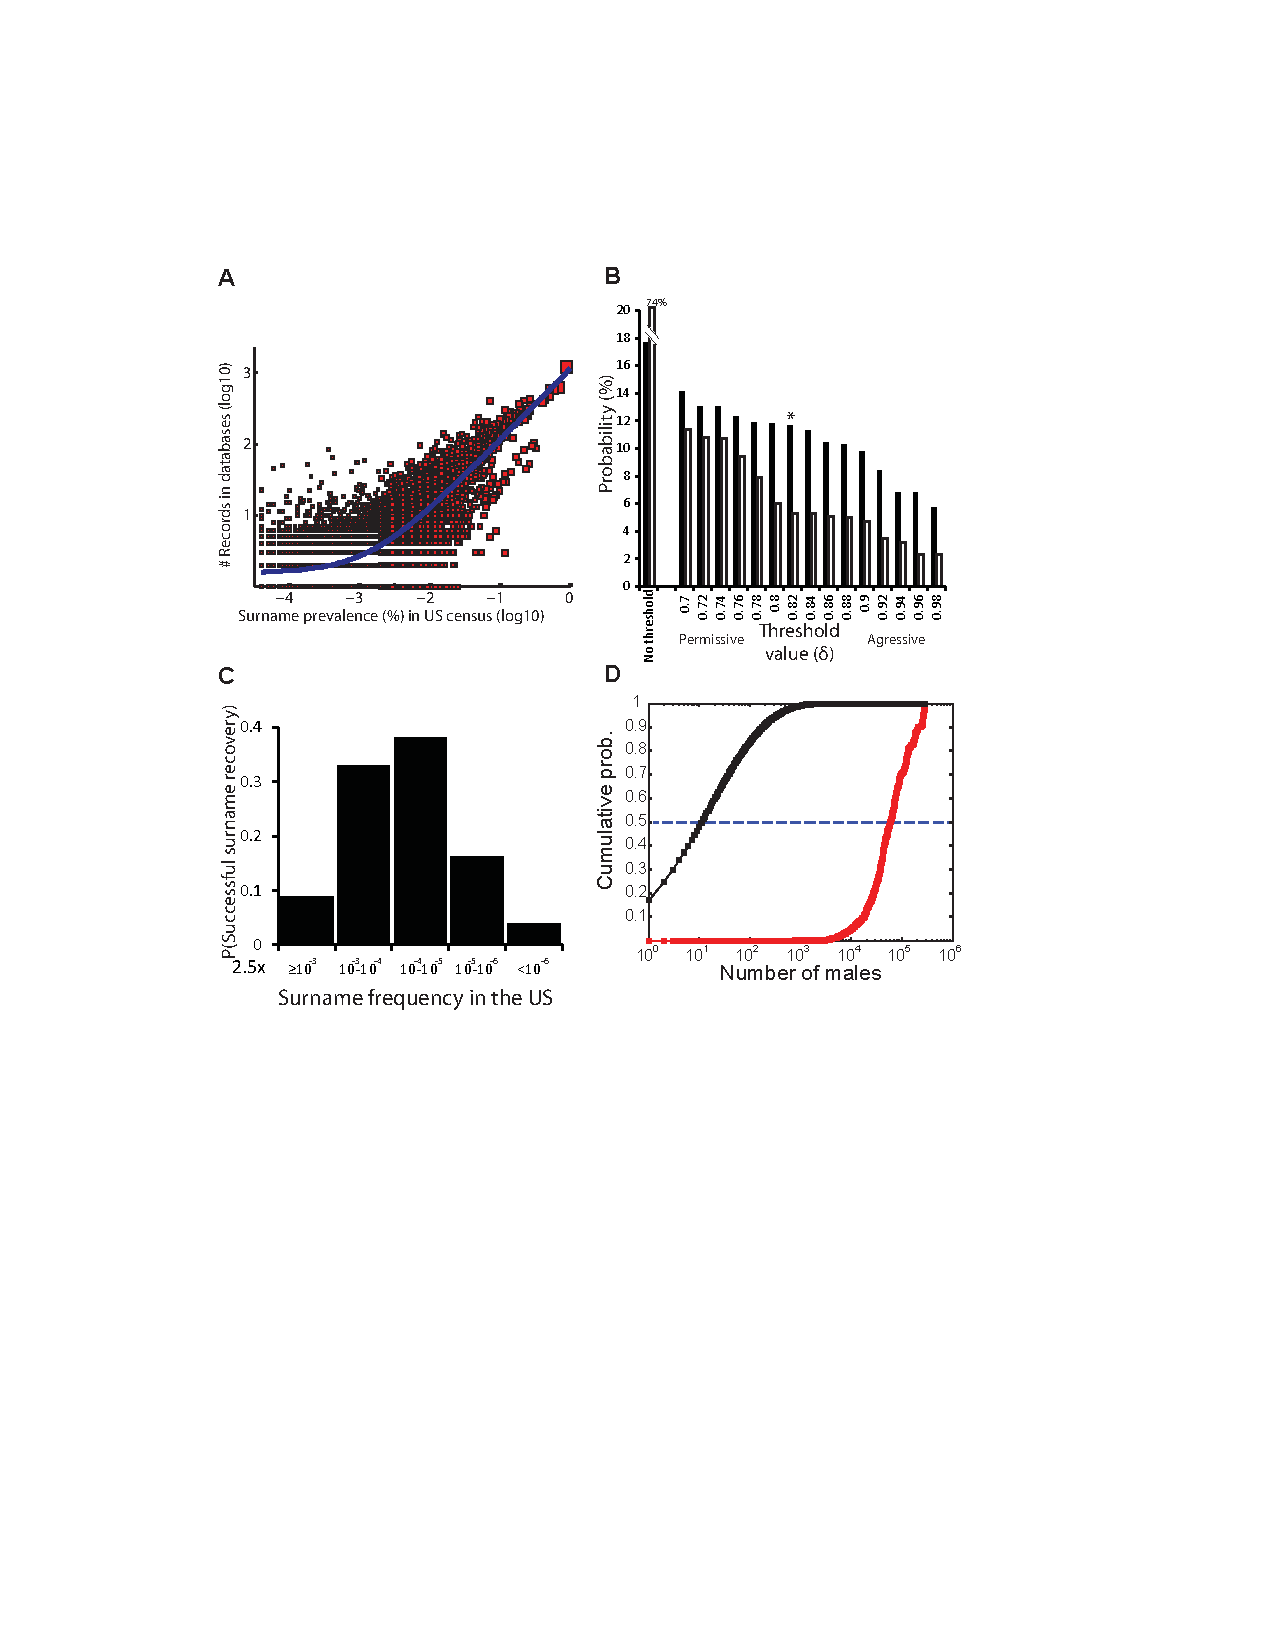
\includegraphics[width=0.5\textwidth]{Figures/App1/Fig1.pdf}
\caption{\textbf{Quantitative assessment of identification via surname inference} \textbf{(A)} The number of Ysearch and SMGF records as a function of surname prevalence in the US population. The best fit line is shown in blue. \textbf{(B)} Expected performance of surname recovery. The probability of successful recovery (closed bars) and wrong recovery (open bars) are shown at different surname confidence thresholds. The star indicates the middle-range performance threshold that was described in the main text. \textbf{(C)} The expected distribution of recovered surnames as a function of their prevalence. Most recovered surnames are expected to have a frequency of 1:4,000 individuals or less. \textbf{(D)} The cumulative distribution function of US males with a profile that matches a specific age, state, and surname combination (black) compared to the distribution when only age and state are known (red). The median is labeled with a dashed line.}
\end{figure}

Next, we established the feasibility of Illumina sequencing to produce accurate Y-STR haplotypes. Using lobSTR, an algorithm for STR profiling from raw sequencing reads \cite{GymrekGolanRossetEtAl2012}, we processed ten high coverage male genomes from the Human Genome Diversity Panel (HGDP). lobSTR produced Y-STR haplotypes with an average length of 53 out of the possible 79 genealogical markers (\textbf{Supplementary Table \ref{fig:sursup5}}). Comparing these results to capillary electrophoresis calls revealed 99\% accuracy. We further found that even at lower sequencing coverage of 10x, informative haplotypes can be obtained by lobSTR (\textbf{Supplementary Figure \ref{fig:sursup4}}). To test the ability to retrieve genetic genealogy records with the Illumina haplotypes, we profiled STRs from the genome of a US Caucasian male from our lab collection that was sequenced with Illumina 100bp reads to a coverage of 13x. In parallel, we submitted this sample to the genealogy service of Sorenson Genomics and created a Ysearch record based on their results. A search with the Illumina haplotype returned his Ysearch entry as a top record (\textbf{Supplementary Figure \ref{fig:sursup5}}).

The NCBI archives host a small number of genomes from identified individuals, providing good test cases for identification via surname inference. We used lobSTR to extract Y-STR haplotypes from the genomes of John West \cite{LeatEhrenreichBenjeddouEtAl2007}, Michael Snyder \cite{LimXueParkinEtAl2007}, and Craig Venter \cite{LevySuttonNgEtAl2007} (\textbf{Supplementary Table \ref{fig:sursup6}}). Searching Ysearch and SMGF with the Y-STR haplotypes of West and Snyder did not return their surnames and resulted in low matches to records with relatively ancient MRCAs 23-28 generations ago (\textbf{Supplementary Material \ref{sec:sursm}}). A search with Craig Venter's haplotype returned a clear match to a ``Venter'' record that was concordant at all 33 comparable markers and with an estimated TMRCA of less than 8 generations (\textbf{Figure \ref{fig:surfig2}}). We further tested whether it would be feasible to trace back Craig Venter by combining his surname with demographic profiling. A query for ``Surname: Venter, Year of Birth: 1946, State: California'' in online public record search engines retrieved two matching records of males, one of whom was Craig Venter himself. 

Surname inference from personal genomes puts the privacy of current de-identified public datasets at risk. We focused on the male genomes in the collection of Utah Residents with Northern and Western European Ancestry (CEU). The informed consent of these individuals did not definitively guarantee their privacy and stated that futuristic techniques might be able to identify them \url{http://hapmap.ncbi.nlm.nih.gov/downloads/elsi/CEPH_Reconsent_Form.pdf}. To test the ability to trace back the identities of these samples from personal genomes, we processed with lobSTR 32 Illumina genomes of CEU male founders that reside in public repositories of the 1000 Genomes Project \cite{AbecasisAltshulerAutonEtAl2010} and the European Nucleotide Archive that were sequenced with read lengths of at least 76bp. Most of these genomes were sequenced to a shallow depth of less than 5x, and produced sparse Y-STR haplotypes. We selected the ten genomes that had the longest Y-STR haplotypes with a range of 34-68 markers to attempt surname recovery. Searching the genetic genealogy databases returned top-matching records with Mormon ancestry in 8 of the 10 individuals for which the top hit had at least 12 comparable markers. Moreover, for four individuals, the top match consisted of multiple records with the same surname, increasing the confidence that the correct surname was retrieved. This potential high surname recovery rate stems from a combination of the deep interest in genetic genealogy among this population and the large family sizes, which exponentially increases the number of targeted individuals for every person that is tested. 

\begin{figure}[h!]
\centering
\label{fig:surfig2}
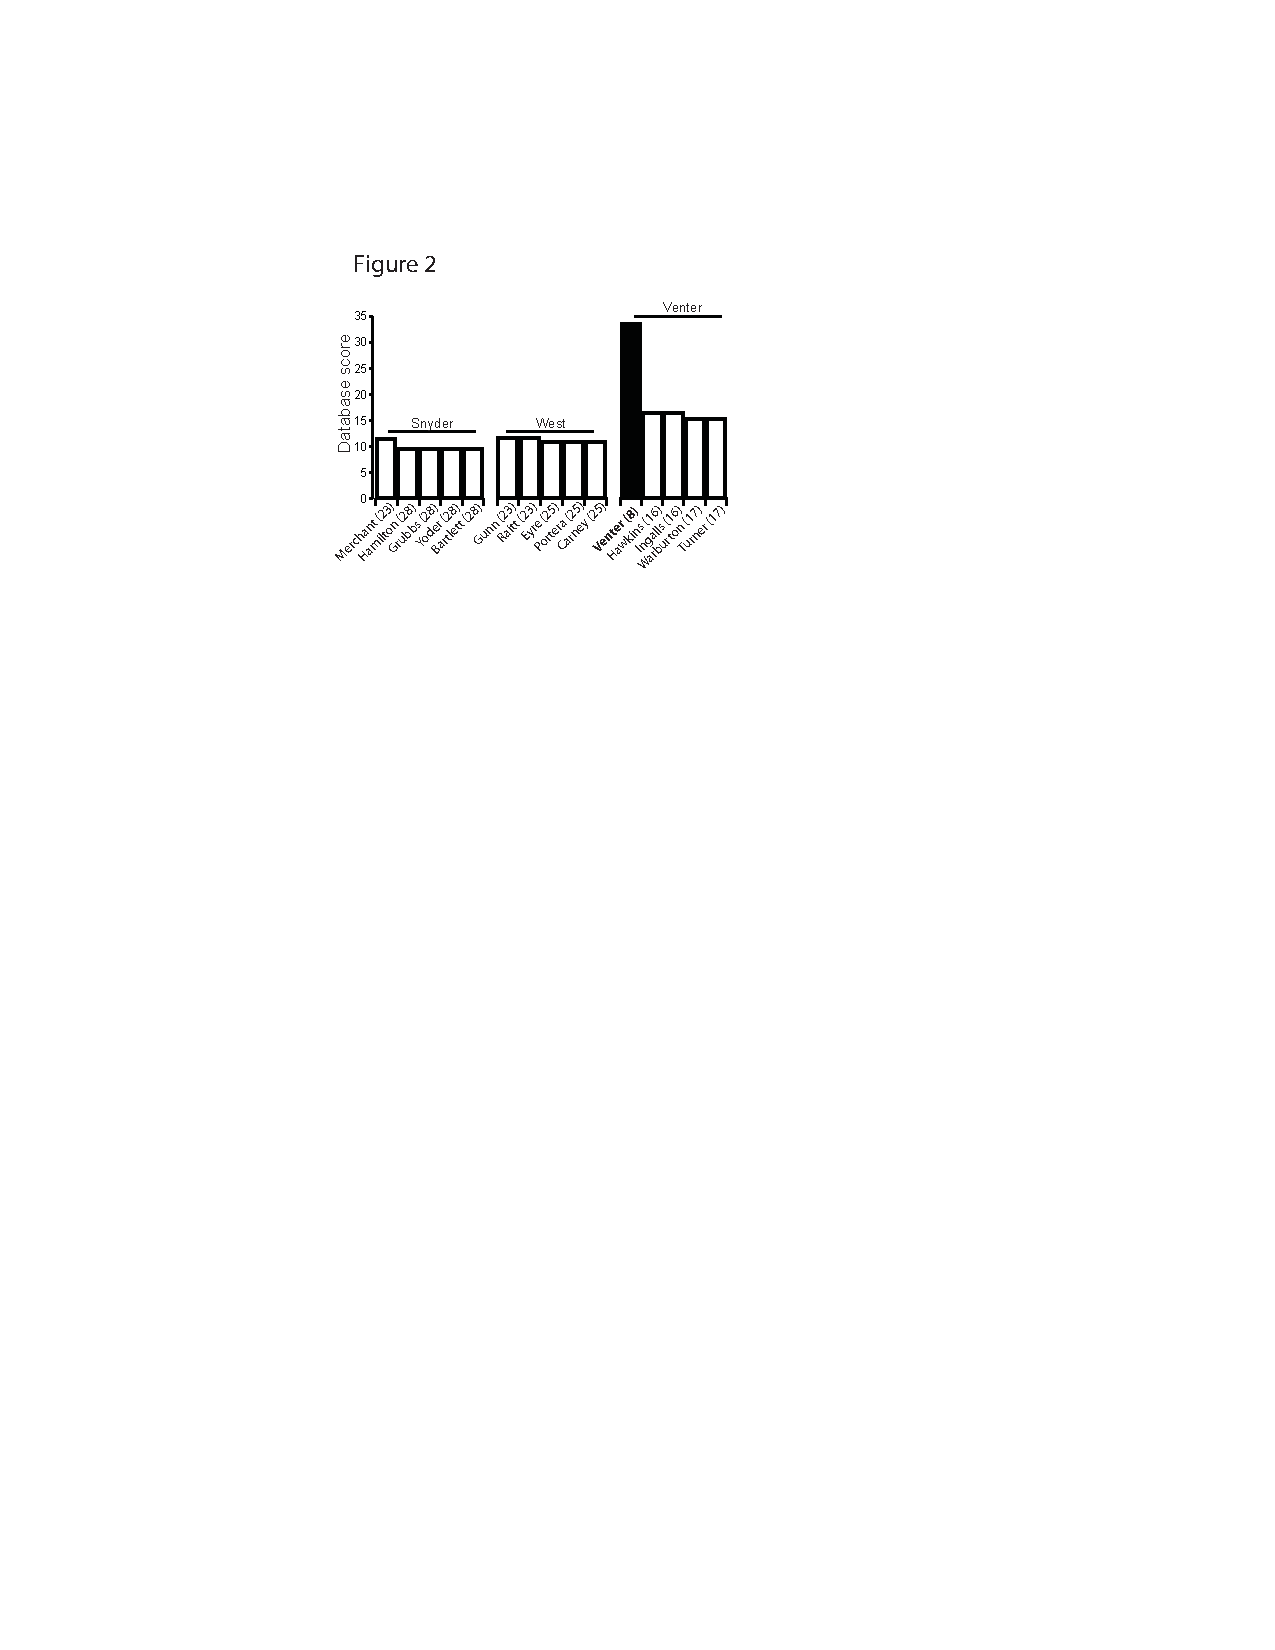
\includegraphics[width=0.5\textwidth]{Figures/App1/Fig2.pdf}
\caption{\textbf{The top five records retrieved after searching Ysearch with the Y-STR haplotypes of Michael Snyder, John West, and Craig Venter.} The expected number of generations to the MRCA is given in parentheses for each record. Searching with Craig Venter returned a ``Venter'' record (closed bar) as the top match.}
\end{figure}

In five surname recovery cases, we fully identified the CEU individuals and their entire families with very high probabilities (\textbf{Table \ref{tab:surtab1}}). These five cases belonged to three pedigrees, where in two of these pedigrees the surnames of both the paternal and maternal grandfathers were recovered. Our strategy for tracing back individuals relied on the recovered surnames as well as publicly available Internet resources such as record search engines, obituaries, and genealogical websites, and demographic metadata available in the Coriell Cell Repository website. The year of birth was inferred by subtracting the ages in Coriell from the year of collecting samples. Each search took 3 to 7 hours by a single person. The identified families matched exactly to the corresponding pedigree descriptions in the Coriell database: the number of children, the birth order of daughters and sons, and the state of residence were identical. All grandparents were alive in 1984, the year that the CEU cell line collection was established \cite{PrescottLalouelLeppert2008}. In the two cases of a dual surname recovery from both grandfathers, the surname of the father and the maiden name of the mother matched exactly to the grandfathers' surnames, substantially increasing the confidence of the recovery. Coriell also lists the ages during sample collection for these two pedigrees, which agreed with the age differences of the identified family members. Using genealogical websites, we traced the patrilineal lineage that connects each identified genome through the MRCA to the record originator in the genetic genealogy database (\textbf{Fig. \ref{fig:surfig3}}). This analysis revealed that two to seven meiosis events link the CEU genome to the record source. Finally, we calculated that the probability of finding random families in the Utah population with these exact demographic characteristics is less than 1 in 105-109 (\textbf{Supplementary Material \ref{sec:sursm}}). In total, surname inference breached the privacy of nearly 50 individuals from these three pedigrees.

This study shows that data release, even of a few markers, by one person can spread through deep genealogical ties and lead to the identification of another person who might have no acquaintance with the person who released his genetic data. The propagation of information through shared male lines amplifies the range of identification, allowing $\sim$135,000 records to potentially target several millions of US males. Another feature of this identification technique is that it entirely relies on free, publicly-available resources. It can be completed end-to-end with only computational tools and an Internet connection. The compatibility of our technique with public record search engines makes it much easier to continue identifying other datasets in the same pedigree, including female genomes, once one male target is identified.  We envision that the risk of surname inference will grow in the future. Genetic genealogy enthusiasts add thousands of records to these databases every month. In addition, the advent of third-generation sequencing platforms with longer reads will enable even higher coverage of Y-STR markers, further strengthening the ability to link haplotypes and surnames.

\begin{figure}[h!]
\centering
\label{fig:surfig3}
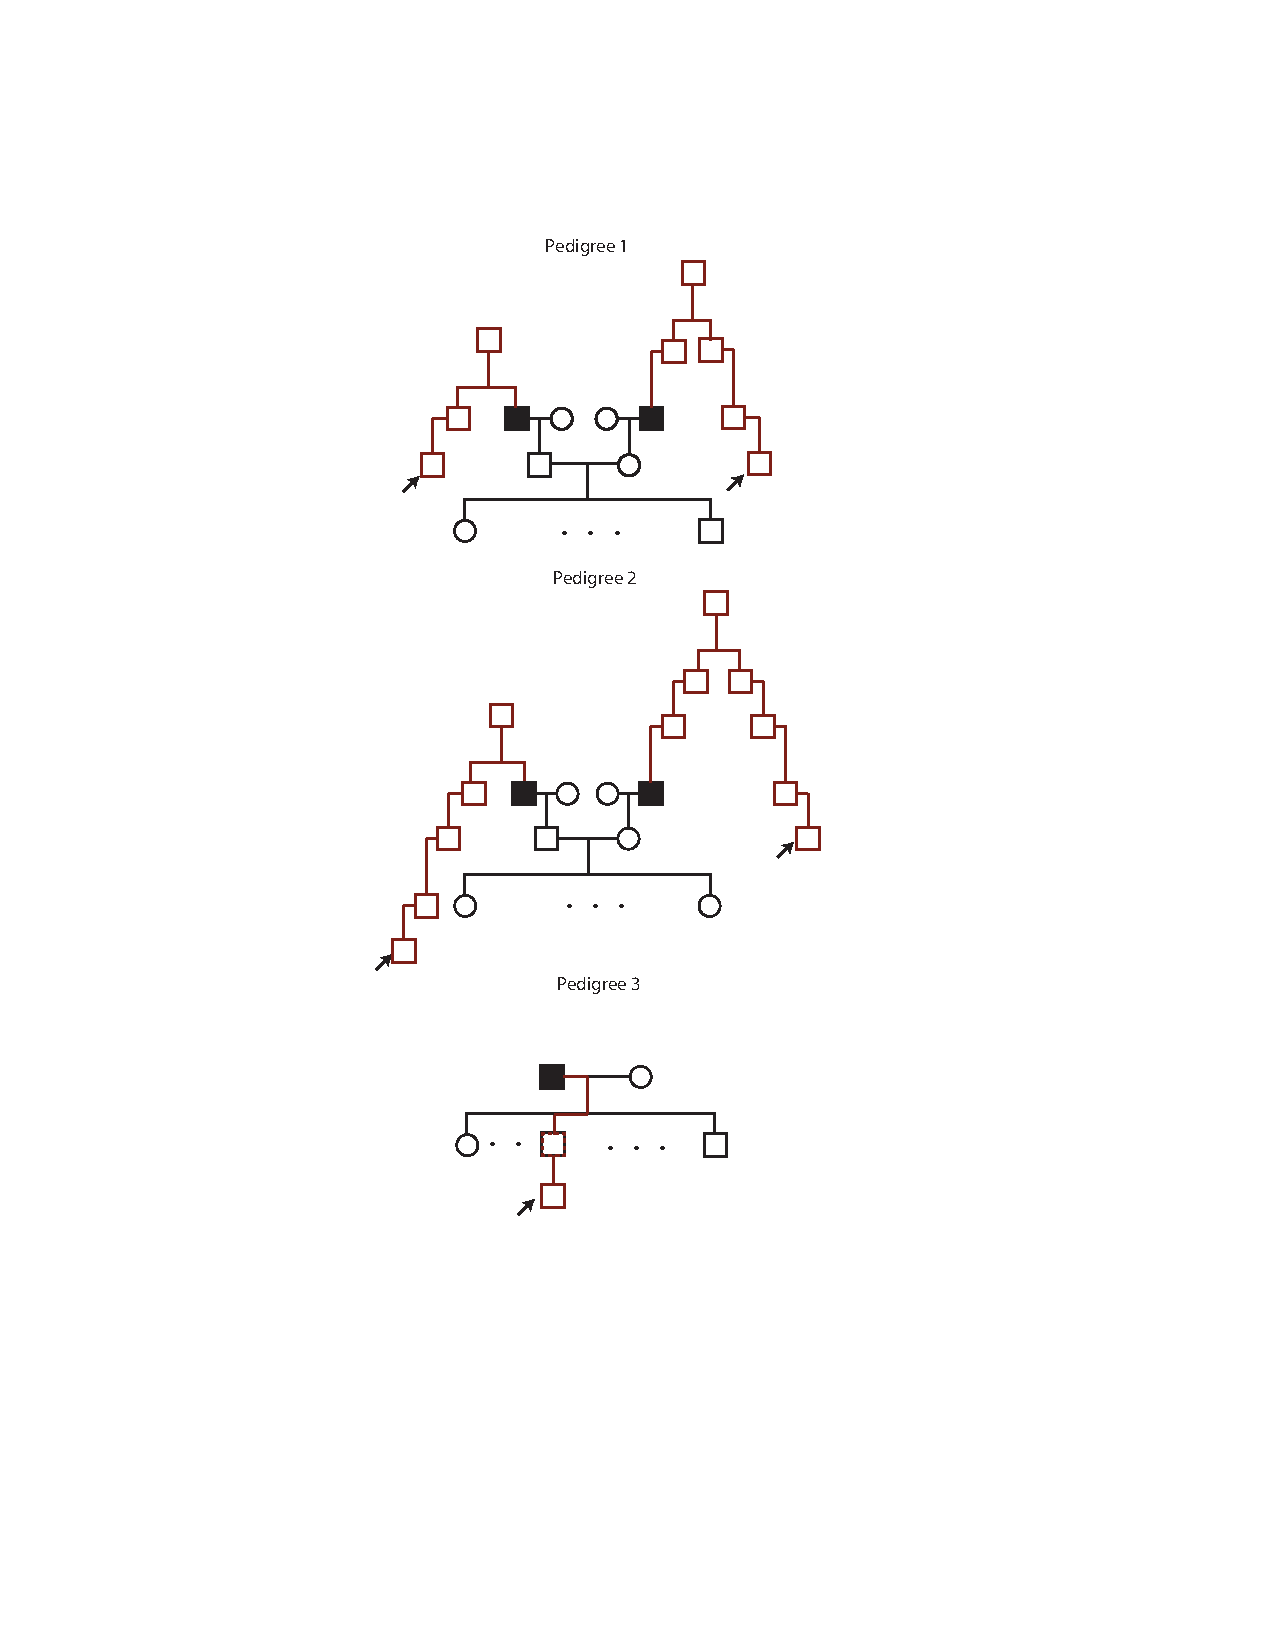
\includegraphics[width=0.5\textwidth]{Figures/App1/Fig3.pdf}
\caption{\textbf{Illustrations of the three CEU pedigrees (black) showing how genetic information from distant patrilineal relatives (arrow; red - patrilineal lines) can identify individuals.} Filled rectangles represent sequenced individuals. To respect the privacy of these families, only abbreviated versions are presented. The sex of the CEU grandchildren was randomized.  The numbers of grandchildren are not given.}
\end{figure}

Similar to other genetic privacy issues \cite{LinOwenAltman2004,BieberBrennerLazer2006,HomerSzelingerRedmanEtAl2008,JacobsYeagerWacholderEtAl2009,ImGamazonNicolaeEtAl2012,CraigGoorWangEtAl2011,SchadtWooHao2012}, preventing surname inference from public whole genome datasets might be quite challenging. Masking Y-STR markers could limit the effectiveness of the method presented in this study, but this approach is not sustainable (\textbf{Supplementary Material \ref{sec:sursm}}). Our analysis suggests that Y-STR haplotypes can be imputed back from SNPs on the Y-chromosome (Y-SNPs) when a large reference set of male genomes will be available (\textbf{Supplementary Figure \ref{fig:sursup6}}). In addition, community efforts, such as the Y Chromosome Genome Comparison, have already started exploring the association between Y-SNPs and surnames (\textbf{Supplementary Table \ref{tab:sursuptab1}}), and might allow bypassing Y-STR masking. We also posit that restricting genetic genealogy information is not practical as some of the data is already scattered in multiple end-user websites and genealogy mailing lists. 

Existing policy tools, such as controlled access databases with data use agreements, may mediate the exposure of genomic information to surname inference. However, in our view, the appropriate response to genetic privacy challenges such as these is not for the public to stop donating samples or for data sharing to stop - which would be devastating reactions that could significantly hamper scientific progress. Rather, we believe that establishing clear policies for data sharing, educating participants about the benefits and risks of genetic studies \cite{McGuireGibbs2006} and the legislation of proper usage of genetic information are pivotal ingredients to support the genomic endeavor.

\begin{figure}[h!]
\centering
\label{tab:surtab1}
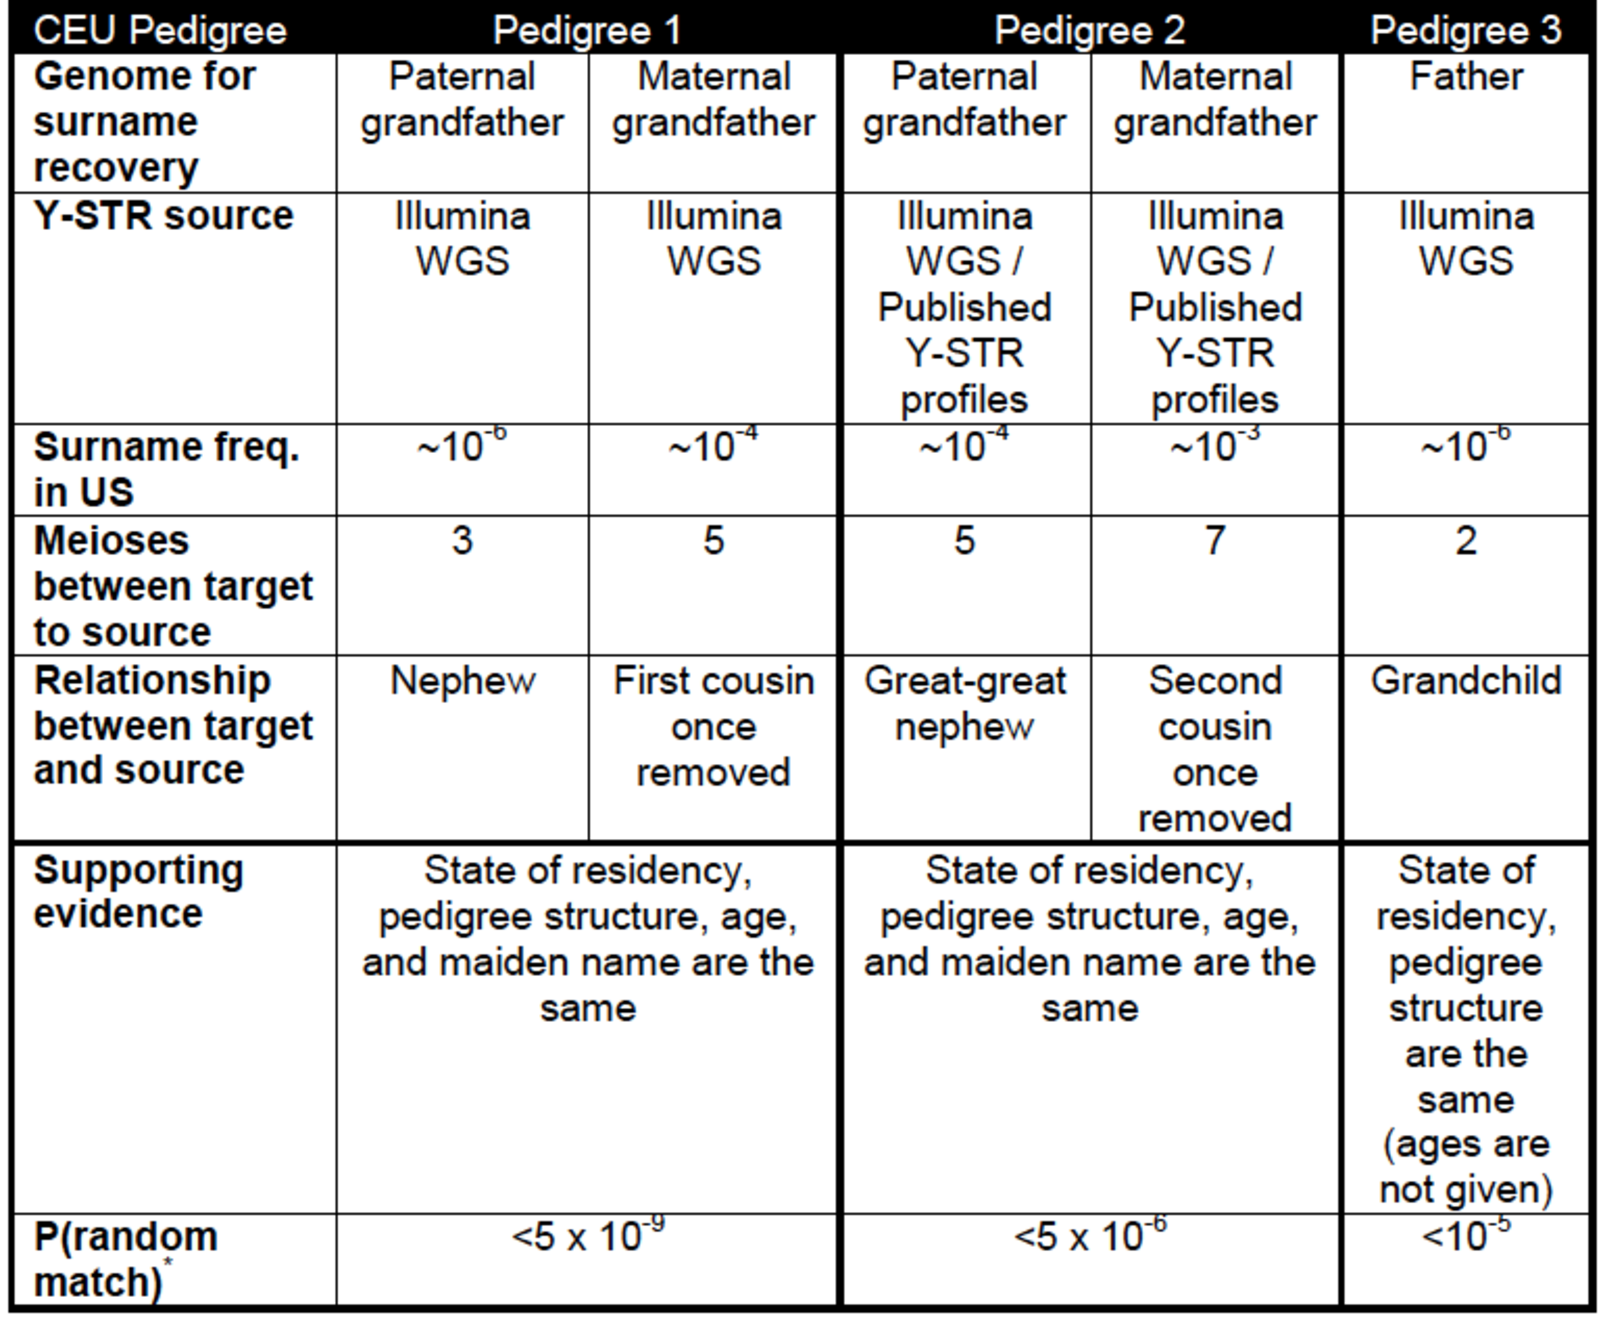
\includegraphics[width=0.9\textwidth]{Figures/App1/Table1.pdf}
\caption{\textbf{Comparison of CEU identification cases.}}
\end{figure}

\section{Acknowledgements}
We thank FamilyTreeDNA and SMGF for technical assistance. The authors would like also to thank Dina Esposito, Alon Goren, Gerry Fink, David Page, Wendy Kramer, and Roy Ronen, for useful discussions. Y.E. is an Andria and Paul Heafy Family Fellow. This publication was supported by the National Defense Science and Engineering Graduate Fellowship (M.G.) and by the Edmond J. Safra Center for Bioinformatics at Tel-Aviv University (D.G. and E.H.). 

\section{Supplementary Material}
\label{sec:sursm}

\subsection{Evaluating the general risk of surname recovery}
\subsubsection{Downloading Ysearch data}
The Ysearch website belongs to FamilyTreeDNA (FTDNA), a Texas-based genetic genealogy company. The website allows users, regardless of their testing service, to voluntarily post their Y-STR genotyping results along with their ancestral information and contact details. Based on the data posted on the website, approximately 85\% of Ysearch's users were tested with FamilyTreeDNA and the other 15\% were tested with other genetic genealogy services. Users from other services are advised to post their results using FamilyTreeDNA nomenclature, and the website offers a conversion table between popular genetic genealogy services and FamilyTreeDNA nomenclature.

With permission from FamilyTreeDNA, we scraped the entire Ysearch database in May 2011. Some areas are protected by reCaptcha and were accessed manually. After parsing and merging the HTML files, we obtained 95,000 surname-haplotype entries, each of which contained: Ysearch userID, surname, ancestral location, and Y-STR results. 

\subsubsection{Access to the SMGF database}
The SMGF website belongs to the Sorenson Molecular Genealogy Foundation, a Utah-based non-profit genetic genealogy organization that was recently acquired by Ancestry.com. The website allows users to query the SMGF database but not to create new records, and all records are from the SMGF program. Unlike the Ysearch database, we could not download the database records to our server. With permission from SMGF, we conducted massive queries of their database using an automatic script. The webpages that contained the top 10 results based on the SMGF matching algorithm were downloaded and parsed to identify the matches. 

\subsubsection{Concordance between genealogical databases and the US population}
The surname distribution in the general US population was estimated using the Census 2000 study that is based on 270 million records (\url{http://www.census.gov/genealogy/www/data/2000surnames/index.html}). The Census study lists 151,671 surnames along with their relative prevalence in the general population and ethnic composition in sorted order. To protect the privacy of the participants and due to sample size limitations, the Census data stops when the cumulative frequency of the surnames reaches 90\%, and does not include surnames that are found in less than 100 individuals each. 

We compared the surname distribution in Ysearch and SMGF to the distribution in the general US population in order to evaluate the completeness of the databases. We defined the census coverage probability, denoted by $c$, as the chance that the surname of an individual drawn at random from the US population has at least a single haplotype record in one of these databases, and found that $c$=68.5\%. The correlation between the US population and the genealogical records was evaluated by a permutation test with 10,000 repetitions. We obtained the following statistics: $E[SSE_{permutations}]=9.01 \times 10^6$, $\sigma(SSE_{permutations})=2437$. The hypothesis $SSE$ was $1.99 \times 10^6$. The p-value was calculated using one-sided Chebyshev bound.

\subsubsection{A mathematical model for surname leakage risk}

\emph{Search method}

Our database search method relied on finding a record that shares the closest Time to Most Recent Common Ancestor (TMRCA) with the queried haplotype. The rationale behind this strategy is that close patrilineal relatives have a higher probability of sharing the same surname. For instance, one can imagine that monozygotic twins have a high probability of sharing the same surname, whereas a pair of Y chromosomes whose MRCA lived before the formation of the surname system would have a low probability of sharing the same surname. 

Walsh \cite{Walsh2001} has proposed several Bayesian models for estimating the distribution of the TMRCA in non-recombining haplotypes. We used his ``infinite alleles model with differential mutation rates''. Consider two Y chromosome haplotypes with $n$ STR loci denoted by $\vec{v}=(v_1,v_2,\hdots,v_n)$ and $\vec{u}=(u_1,u_2,\hdots,u_n)$, with vector elements corresponding to the allele lengths. Let $\vec{x} = (x_1,x_2,\hdots,x_n)$ be a binary vector with $x_i=1$ for a match at the $i$-th locus of $\vec{v}$ and $\vec{u}$, and $x_i=0$ otherwise, and let $\vec{\mu}=(\mu_1,\mu_2,\hdots,\mu_n)$ be a vector whose elements denote the probability of a mutation per meiosis in each marker. According to Walsh's model, the probability distribution function (PDF) of the TMRCA between the two haplotypes is:

\begin{equation}
\label{eq:sureq1}
P(t|\vec{x},\vec{\mu}, N_e) = \frac{e^{-t(\frac{1}{N_e}+2\sum_{i=1}^n\mu_ix_i)}\Pi_{i=1}^n(1-e^{-2t\mu_i})^{(1-x_i)}}{I(\vec{x},\vec{\mu},N_e)}
\end{equation}

where $N_e$ is the effective male population size, and $I$ is a normalization factor to ensure that $\sum_{t=0}^{\infty}P(t|\vec{x},\vec{\mu},N_e)=1$. Following Thomson et al. \cite{ThomsonPritchardShenEtAl2000}, $N_e$ was set to 10,000 males. The mutation rates were obtained from the extensive study of Ballantyne, et al \cite{BallantyneGoedbloedFangEtAl2010}.

The expected TMRCA is denoted by τ and is given by:

\begin{equation}
\tau = \sum_{t=0}^{\infty}t_i P(t_i|\vec{x}, \vec{\mu}, N_e)
\end{equation}

The recovered surname was selected according to the record that has the minimal $\tau$ to the searched haplotype. Due to technical constraints with the web queries to SMGF and in order to reduce the amount of calculations, we did not determine $\tau$ for each of the hundreds of thousands of users in the databases. Instead, we employed the following procedure: (i) Ysearch - identify a set of candidate records that have the maximal number of matching markers to the queried haplotype (ii) SMGF – use the native SMGF search tool to identify the top 10 candidates according to the website's proprietary algorithm (iii) Both – calculate $\tau$ for top candidates in Ysearch and SMGF using Eq. \ref{eq:sureq1}, and select the record with the minimal $\tau$ of the searched haplotype. 

\emph{Retrieval confidence score}

The retrieval confidence score determined the probability that the TMRCA of the retrieved record is indeed shorter than that of (i) a record with a distinct surname that has the second to shortest TMRCA and (ii) a random person from the population. Let $P_1$ and $P_2$ be the TMRCA PDFs of the best record and second best record according to Eq. \ref{eq:sureq1}, and let P3 be the PDF of coalescent in a Fisher-Wright population: $P_3 (t|N_e)=N_e^{-1} e^{-N_e t}$. In addition, let $F_i$ be the cumulative probability distribution function of $P_i$. The retrieval confidence score, $\delta$, is given by:

\begin{equation}
\delta(P_1,P_2,P_e) = \sum_{j_1=1}^TP_1(j_1)
\Bigg(
\sum_{j_2>j_1}^TP_2(j_2)
 \Big(
 \sum_{j_3>j_1}^TP_3(j_3)
 \Big)
\Bigg) = \sum_{j=1}^TP_1(j)(1-F_2(j))(1-F_3(j))
\end{equation}

$T$ is the number of generations that is practical for the patrilineal surname system and was set to 20 generations, corresponding to $\sim$1400 AD. $P_2$ was obtained by scanning records in the list that was generated in step (iii); candidate records with less than 20 markers were excluded as well as records with surnames that matched the top hit.

\emph{Surname inference}

We set a threshold, $\delta_0$, which denotes the minimal accepted quality for valid surname recovery. If the retrieval passed the confidence threshold, the algorithm inferred that the record's surname is the surname of the input haplotype. Otherwise, the algorithm rejected the inference and returned ``Unknown''. 1.8\% of the searches returned records with an empty surname field or with strings that are not found in the surname list of the US census such as ``AshkenaziJewishModal''. The algorithm reported these cases as ``Unknown'' as well. Finally, TMRCA ties between two or more records with distinct surnames were also treated as ``Unknown''. 

A surname inference resulted in one of the following outcomes: success – the recovered surname is concordant with the true surname, wrong – the recovered surname does not match the true surname, unknown – below confidence threshold, non-valid surnames, and ties.  

Following previous record linkage studies \cite{GrannisOverhageMcDonald2004,Winkler1995}, successful recoveries included a small number of cases where the returned surname displayed a minute spelling variant from the true one, such as Abernathy and Abernethy. These cases can still direct the adversary in tracing back the target at the price of searching for a larger number of individuals. We adopted a stringent approach to detect spelling variants that required that the first letter of both surnames be identical and that the Jaro-Winkler string distance \cite{Winkler1995} of the surnames be at least 0.9. This relies on the observation that the suffix of a surname is more prone to mutate than the prefix \cite{Winkler1995}. Two percent of the queries showed spelling variants using this approach and they are summarized in the following table:

\begin{table}[h!]
\begin{tabular}{|l|l|l|}
\hline
True surname & Retrieved surname & Jaro-Winkler distance \\
\hline
ABERNATHY    & ABERNETHY    & 0.977 \\
AYRES        & AYERS        & 0.96  \\
BAIRD        & BEARD        & 0.933 \\
BRALLEY      & BRAWLEY      & 0.947 \\
BRITTON      & BRITTAIN     & 0.944 \\
CHRISTIE     & CHRISTISON   & 0.94  \\
CLARK        & CLARKE       & 0.967 \\
COLLISON     & CULLISON     & 0.964 \\
DENNEY       & DENNY        & 0.967 \\
DUFF         & DUFFEL       & 0.933 \\
FLICKINGER   & FLUCKIGER    & 0.93  \\
MCMURTRY     & MCMURTREY    & 0.984 \\
MILLICAN     & MILLIKEN     & 0.937 \\
PALLETT      & PARLETTE     & 0.919 \\
PARLET       & PARLETTE     & 0.956 \\
SAYRE        & SAYER        & 0.961 \\
SEELYE       & SEELY        & 0.967 \\
WETHERINGTON & WITHERINGTON & 0.961 \\
\hline
\end{tabular}
\end{table}

Manual inspection of the genealogical records showed that in a large number of these cases the users indicated the spelling variant as an alternative ancestral surname.

The general risk of surname leakage from personal genomes is dictated by three factors: the prior distribution of surnames in personal genomes datasets, the distribution of haplotypes within a surname, and the ability to successfully retrieve the surname from the database using the haplotype. For simplicity, we assumed that the distribution of surnames of personal genomes is similar to the distribution of surnames in the population. 

Let $I_x(h,s)$ be an indicator function that returns 1 if querying the database with the combination of haplotype $h$ and surname s returns the outcome $x$, where $x$ is either: ``success'', ``wrong'', or ``unknown''. Let $f_s$ be the frequency of a surname and α(h,s) be the frequency of haplotype $h$ in the surname $s$. Define $\beta_x(s) = \sum_{h \in H(s)} \alpha(h,s)I_x(h,s)$, where $H(s)$ is the set of haplotypes that are associated with the surname $s$. The probability of the surname recovery outcome x for a given population is:

\begin{equation}
\label{eq:sureq3}
P(x) = \frac
{\sum_{s \in S} f_s \beta_x(s)}
{\sum_{s \in S} f_s}
\end{equation}

Where $S$ is the set of all surnames in the population. The probability in Eq. \ref{eq:sureq3} can be assessed by sampling individuals from the population using the following estimator:

\begin{equation}
\label{eq:sureq4}
P(x) = 
\frac{\sum_{s \in S} \hat{f}_s \hat{\beta}_x(s)}
{\sum_{s \in S}\hat{f}_s}c + 
\frac{\sum_{s \in \overline{S}} \hat{f}_s\hat{\beta}_x(s)}
{\sum_{s \in \overline{S}} \hat{f}_s} (1-c)
\end{equation}

where $S$ is the set of surnames in the sample that are known to be present in the tested databases and $\overline{S}$ is the set of surnames in the sample that are known to be absent from the tested databases. $\hat{f}_s$ is the estimated frequency of the surname based on the Census data, $\hat{\beta}_x(s) = \sum_{h \in H(s)} \hat{\alpha}(h,s)I_x(h,s)$ and $\hat{\alpha}(h,s)$  is the frequency of the haplotype-surname combination in the sample, and $c$ is the census coverage probability that was determined above. Eq. \ref{eq:sureq4} models the outcome rates as a weighted sum of sampling individuals from two distinct strata: those whose surname is found in the databases and those who do not. The two weights mitigate potential ascertainment biases in the sample and increase the confidence that the results reflect the target population.

\subsubsection{Estimating the risk of surname leakage by inter-database comparisons}
Our input sample relied on a cohort of individuals from the YBase database. This database was maintained by DNA Heritage and was acquired by FamilyTreeDNA in April 2011. FamilyTreeDNA provided us with surname-haplotype records from the database, without other identifiers that can expose the identity of the database users. The YBase and SMGF entries are completely distinct because the SMGF database lists only SMGF users. We took the following steps to remove potential duplicate records between Ysearch and Ybase: first, we asked FamilyTreeDNA to exclude YBase entries whose email addresses appear in Ysearch as well as entries without email addresses. Second, we removed from the downloaded copy of Ysearch all $\sim$900 users that were tested with DNA Heritage. Third, we excluded any YBase user whose haplotype did not show a combination of markers that are typical to the DNA Heritage test panel. Thus, the input cohort was tested with a different company (DNA Heritage) than the database users. This reduces the chance of ascertainment biases due to oversampling of close relatives of the database participants.

Genetic genealogy databases are subject to nomenclature heterogeneity that can confound the analysis. This is especially problematic for DNA Heritage test panels that were subject to five nomenclature changes between 2003 to 2009 (see: \url{http://web.archive.org/web/20100307032155/http://www.dnaheritage.com/helpfiles/DNA_Heritage_nomenclature_changes.pdf}). For each input haplotype, we inspected the allelic ranges for markers that underwent significant nomenclature changes, such as DYS452, to decipher the nomenclature stratum and to standardize the haplotype according to the NIST recommended nomenclature. In addition, we set a tolerable genotype range for each marker that is equal to the marker mean value in Ysearch$\pm$3std. Entries outside of this range have a high likelihood of nomenclature differences and typos of users. This step filtered approximately 5\% of YBase haplotypes. Finally, we selected only YBase haplotypes that have full genotyping results for a set of 34 STR markers (\textbf{Supplementary Table \ref{tab:sursuptab2}}) and whose surnames are in the US census. At the end of this process, we retained 911 YBase records.

We used a series of Perl scripts to challenge Ysearch and SMGF with the YBase haplotypes and to compare the returned surnames to the true ones. SMGF searches were conducted with the NIST nomenclature and Ysearch searches were conducted with FamilyTreeDNA nomenclature. The standard deviation was calculated by 30 iterations of re-sampling with replacement participants from the input cohort and repeating the analysis process.

The results of the 911 queries exhibited distinct patterns between the TMRCA of records that exactly match the true surname, records with a spelling variant, and records that returned the wrong surnames (\textbf{Supplementary Figure \ref{fig:sursup1}}). The mean TMRCA was 10.3 generations for exact matches, 15.6 generations for a spelling variant, and 24.3 generations for wrong surnames. The TMRCA distribution of exact matches appeared to follow a geometric distribution trend. The TRMCA of records with spelling variants was almost never more recent than 10 generations and was quite different from the distribution of wrong matches. This provides another support for our spelling variations detection algorithm. \textbf{Supplementary Figure \ref{fig:sursup2}} shows the final results after processing the results according to Eq. \ref{eq:sureq4}.

\subsection{From Surnames To Individuals}
\subsubsection{The frequency distribution of leaked surnames}
We determined the frequency distribution of leaked surnames from the YBase simulations using the following equation:

\begin{equation}
\label{eq:sureq5}
P(s \in S_i | x = success, \delta) = \frac
{P(x=success | s \in S_i, \delta)P(s \in S_i)}
{P(x=success | \delta)}
\end{equation}

Where $S_i$ is a subset of surnames whose frequencies fall in the $i$-th bin out of $j$ possible bins. Specifically, we used the following bins:

\begin{table}[h!]
\begin{tabular}{|l|l|l|}
\hline
Bin(i) & Frequency boudnaries & Example of surnames in bin \\
\hline
1& 	$>$1:400 &	Smith, Johnson \\
2	&1:400 – 1:4,000	& Turner, Collins\\
3	& 1:4,000 – 1:40,000 & 	Gates, Sloan\\
4	& 1:40,000 – 1:400,000 &	Bjork, Reach \\
5	& $<$1:400,000 &	Kellog, Venter \\
\hline
\end{tabular}
\end{table}

The term $P(s \in S_i)$ in Eq. \ref{eq:sureq5} is given by the census data. The other numerator term can be approximated using a slight modification to Eq. \ref{eq:sureq4}:

\begin{equation}
\label{eq:sureq6}
P(x = success | s \in S_i, \delta) = 
\frac{\sum_{s \in S} \hat{f}_s \hat{\beta}_x(s)}
{\sum_{s \in S}\hat{f}_s}c_i + 
\frac{\sum_{s \in \overline{S}} \hat{f}_s\hat{\beta}_x(s)}
{\sum_{s \in \overline{S}} \hat{f}_s} (1-c_i)
\end{equation}

Where $c_i$ is a normalization factor that denotes the probability that a random person from the US population whose surname is in the $i$-th bin has at least a single entry in Ysearch and SMGF.  $c_i$ was determined by intersecting the census data with the list of Ysearch and SMGF. We used $\delta$=0.82.

The leaked surnames are mostly found in the intermediate bin with a frequency of 1:4,000-1:40,000. Extremely rare surnames have the lowest relative risk for leakage due to the absence of records in Ysearch and SMGF. However, if these databases have even a single record for an extremely rare surname, then there is a 43\% chance that the surname will be exposed (\textbf{Supplementary Figure \ref{fig:sursup3}}). This phenomenon is potentially due to the small number of male lineages in extremely rare surnames.	

\subsubsection{Combining surnames with demographic identifiers}
The joint probabilities of sex, age, and state were obtained from the US Census Population Estimates Program (\url{www.census.gov/popest/states/asrh/files/SC-EST2009-AGESEX-RES.csv}). The data is based on Census 2000 and contains a projection of residents to 2009, which was used in the simulation. Similar to the HIPAA law, ages that are over 85 were grouped in a single category. 

The simulation ran 100,000 times. In each round, a combination of state and age was selected according to their probability in the joint distribution. For instance, there are 287,000 males in California who are 25 years old and 3,500 males in Idaho who are 75 years old. Accordingly, the probability of selecting ``California, 25'' was 82 times higher than selecting ``Idaho, 75''. Next, a bin of a leaked surname was selected according to its probability in Eq. \ref{eq:sureq6} and a surname was selected according to its frequency in the bin. For instance, in the case of selecting the 1st bin ($\geq$1:400), Smith had 1.28 higher probability of being sampled than Johnson. Finally, the simulation randomly selected between the return of a spelling variant or exact match, where the former had a probability 11.11\%, based on our empirical findings in the Ybase simulations. In case of no spelling variant, the surname frequency was set to the census frequency; otherwise, the surname frequency was selected to be the sum of frequencies of all surnames that can be spelling variants of the original surname according to our spelling variant definition above. The last step portrays a scenario in which the adversary first looks for the target with the returned surname and if he cannot trace the target back, he tries all spelling variants. The number of expected individuals was found by multiplying the surname frequency by the number of males with the selected age and geographical location.

We validated the results of the simulation by comparing them to real datasets of US residents from PeopleFinders (\url{www.peoplefinders.com}). These datasets are based on extensive mining of public records, such as voter and drivers license registries, and can be searched by a combination of surname, age, and state. We selected 30 random simulation rounds that passed two criteria: (a) the ages were restricted to 25-35 years to avoid potential confounding due to underrepresentation of minors in public records and conflicting records from deceased individuals (b) the expected number of individuals should be 10-100 to avoid overloading the website. In most cases the lists in PeopleFinders were smaller than expected from simulations. Although we cannot rule out incompleteness of the website, the results also suggest that any underestimation of the list size - if it exists at all - is not significant.

\subsection{Profiling Y-STRs from sequencing data}
\subsubsection{lobSTR usage}
Unless otherwise specified, lobSTR v2.0.0 was used to profile Y-STRs from raw whole-genome sequencing data \cite{GymrekGolanRossetEtAl2012}. In brief, lobSTR acts in three steps: detecting reads with repetitive elements that are flanked with non-repetitive regions, aligning the flanking regions to a reference, and measuring the repeat length for each STR. 

\emph{Improved Y-STR reference}

We modified lobSTR's standard STR reference to include the genomic locations and nomenclatures of genealogical Y-STRs. These locations were found by conducting in silico PCR on the UCSC genome browser using published Y-STR primers \cite{KayserKittlerErlerEtAl2004,BoschLeeCalafellEtAl2002,ButlerDeckerValloneEtAl2006,HansonBerdosBallantyne2006,LimXueParkinEtAl2007,LeatEhrenreichBenjeddouEtAl2007,MalaspinaCiminelliViggianoEtAl1997,SchoskeValloneKlineEtAl2004,JoblingSamaraPandyaEtAl1996} and by searching the FamilyTreeDNA Y chromosome browser (\url{ymap.ftdna.com}). Several STR markers reside in duplicated regions of the Y chromosome. For instance, DYS385 has two distinct alleles in a single individual. Since lobSTR filters multi-mappers, we kept only one entry of these markers in the modified reference. Markers DYS448 and DYS449 consist of two STR regions separated by a non-repetitive region. For these, a separate reference entry was created for each region and the final genotype was determined by adding the alleles profiled at each of the two STR regions. 

We did not include eight genealogical markers in the reference due to various technical reasons: markers GAAT1B07 and DYS724a/b (also known as CDYa/b) were excluded because their corresponding genomic coordinates could not be determined despite extensive literature searches.  DYS726 was excluded because the genetic genealogy nomenclature could not be determined. DYS425 is one of the four repetitive loci of DYF371 \cite{JoblingSamaraPandyaEtAl1996}, and using short reads we could not uniquely determine which locus a read originated from. DXYS156-Y was excluded because it is not specific to the Y-chromosome. Marker DYS19b was not included in because it is present in 0.2\% of the population. Marker DYS640 was incorrectly annotated in our original reference and discarded from further analysis. Marker DYS464a-d was excluded because in most cases we typed fewer than four alleles and could not accurately assign typed alleles to forms a-d.  In summary, our reference included 34 out of the 36 markers used by the SMGF panel and 79 out of the 87 markers in the most comprehensive test panel of FamilyTreeDNA. The genomic coordinates and conventions used for each Y-STR are given in \textbf{Supplementary Table \ref{tab:sursuptab3}}). All coordinates reported in this study follow the hg19 human reference build.

\emph{Processing lobSTR calls}

lobSTR returns base pair length differences from the UCSC genome reference. Genetic genealogy services use an STR nomenclature that follows the PCR product sizes according to arbitrary primers \cite{GusmaoButlerCarracedoEtAl2006}. Whenever available we used the NIST nomenclature to translate lobSTR results (\url{http://www.cstl.nist.gov/strbase/ystr_fact.htm}). For searches in the Ysearch database results were converted to FamilyTreeDNA nomenclature using a conversion table available from SMGF (\url{http://www.smgf.org/ychromosome/marker_standards.jspx}). 

For Y-STRs with a single genomic location, the allele with the modal number of supporting reads was used. Y-STR alleles that showed a non-integer number of repeat copies were discarded. We manually inspected a small number of calls where the modal allele was supported by less than 60\% of reads aligned to the locus and enhanced the call by removing reads likely to be erroneous, such as reads that contain a high number of sequence mismatches, reads in which the STR resides towards the end of the read, or reads supporting alleles outside the normal range. Importantly, this procedure was executed completely blind to the true allele if it was known. For bi-mapper markers, such as DYS413a/b, the shortest repeat length was assigned to allele ``a'' and the next to allele ``b''. 

\subsubsection{Comparing lobSTR to the CEPH Y-STR panel}

\emph{General approach}

Sequence data for the CEPH panel were downloaded from the NCBI Short Read Archive from experiment SRP009145, sample SRS269343, runs SRX103805-130812. The sample included 10 HGDP individuals: HGDP00456 (Mbuti Pygmy), HGDP00665 (Sardinian), HGDP01284 (Mandenka), HGDP00542 (Papuan), HGDP00521 (French), HGDP00778 (Han Chinese), HGDP01307 (Dai), HGDP00927 (Yoruba), HGDP01029 (San), HGDP00998 (Karitiana). Autosomal coverage was calculated using the samtools \cite{LiHandsakerWysokerEtAl2009} depth tool and gives the average depth of covered bases based on alignments using BWA \cite{LiDurbin2009a}. lobSTR 2.0.0 with the improved Y-STR panel was used for the analysis.

Genotypes for 76 Y-STRs typed by capillary electrophoresis for the 10 HGDP samples were obtained from the CEPH website (\url{ftp://ftp.cephb.fr/hgdp_supp9/}). Forty-seven of these markers overlapped with the lobSTR reference and were used to evaluate lobSTR's ability to type Y-STRs.

lobSTR reports alleles as the length difference from the UCSC, whereas the CEPH genotypes are reported as the number of repeat copies at each locus. To convert lobSTR output to the same format, we used for following equation: $r+l/p$, where $r$ is the number of base pairs of the STR of the lobSTR reference, $l$ is the reported lobSTR allele in base-pairs, and $p$ is the period of the Y-STR. For all individuals in which lobSTR recovered a genotype for DYS385a/b, only a single allele was returned. If the returned allele matched either the ``a'' or ``b'' form reported by CEPH, it was considered as correct. This follows our search strategy with the personal genomes, where these partial calls of multi-allelic markers were used to exclude matches not containing the lobSTR call for either allele. 

We noticed that the lobSTR calls for all six individuals typed for DYS481 and all three individuals typed for DYS594 are exactly one repeat away from the results in the CEPH study. There is known nomenclature heterogeneity for these markers and some test kits report them with one shorter repeat than as reported by the NIST standard . Concordantly, we converted lobSTR calls to the shorter allele nomenclature to match that reported by CEPH.

\emph{Number of markers profiled at different sequencing coverage levels}

Based on our previous experience with lobSTR, we assumed that STR coverage is linearly related to autosomal coverage. For each genome, we used the Picard (\url{http://picard.sourceforge.net}) DownsampleSam tool to randomly down-sample reads from the lobSTR alignment file to simulate coverage levels corresponding to autosomal coverage ranging from 1x to 25x. For each coverage level, we repeated the lobSTR allelotyping step to call the Y-STRs. The best-fit saturation curve was found using nonlinear least squares to fit a hyperbolic curve and was extended to predict haplotype lengths for up to 50x coverage.

\emph{Further investigation of wrong Y-STR calls}

In our previous studies, we found that PCR stutter noise is a major source of error in calling STR alleles. This type of noise usually adds or subtracts a single repeat unit from the true allele. We noticed that the erroneous calls in DYS490 and DYS572 are several repeats away from the true allele, reducing the probability that these errors stem from stutter noise. Further analysis found that these two markers have X chromosome homologs, and that the calling errors can be attributed to misalignment of the X chromosome STRs. We also noticed that these markers were occasionally detected in the female genomes of the CEU panel, which provides further support for this hypothesis. Future algorithm improvements can use the homolog calls from the X chromosome to detect these errors.

\subsection{Cases of Surname Leakage from Personal Genomes}
\subsubsection{Querying genealogical databases}
In all surname recovery experiments from personal genomes, database queries utilized the native search interfaces of the websites. 

Ysearch was queried using the haplotype matching tool available at \url{http://www.ysearch.org/search_search.asp?uid=&freeentry=true}. Online searches were conducted with the default parameters and using the FamilyTreeDNA nomenclature. SMGF was queried using the tool at \url{http://www.smgf.org/ychromosome/search.jspx} with the options ``Search by Match\%) = 85\%'' using the NIST nomenclature.

\subsubsection{Feasibility of record retrievals with Illumina}
\emph{The US male sample from our lab collection}

The sequencing experiment was approved by the MIT Committee on the Use of Humans as Experimental Subjects (COUHES).  To comply with the COUHES approval, we cannot share the specific Y-STR results, since this could lead to identification of the individual. As an alternative, we provide summary statistics of the length distribution of the detected Y-STR makers. 

Four Catch-All buccal swabs (Epicentre, QEC89100) were used to collect the sample according to the manufacturer's protocol. Genomic DNA was obtained by QuickExtract (Epicentre), followed by phenol-chloroform purification and ethanol precipitation. Library preparation was performed according to the standard Illumina protocol. Three runs of 101bp paired-end reads were generated with a GAIIx platform, generating 740 million reads. Autosomal coverage of 13x (after removing PCR duplicates) was measured using a conventional alignment pipeline as previously described \cite{ErlichEdvardsonHodgesEtAl2011}.  \textbf{Supplementary Figure \ref{fig:sursup4}A} shows the overlap between the markers that were detected by Illumina versus the genealogical profile from Sorenson Genomics. textbf{Supplementary Figure \ref{fig:sursup4}B} shows the number of STRs that were detected using Illumina and Sorenson as a function of their lengths. 

\emph{Database retrieval}

For the 10 HGDP samples and the US male sample, we supplemented our downloaded copy of the Ysearch database with capillary electrophoresis results. Retrieval of records was conducted with the same scripts used for the Y-STR simulations described above. As an additional validation for our results, we created a Ysearch record for the US male using the Ysearch.org website that does not disclose the true surname of the sample and consists of the Y-STR makers that are shared between Sorenson Genomics and Ysearch. Again, a search with the default website interface returned our sample as the top match.

\subsubsection{Analyzing Michael Snyder's genome}
Raw reads for the blood-derived and saliva-derived DNA of Michael Snyder's genome were downloaded from the NCBI Sequence Read Archive with accessions SRX097307 and SRX097312, respectively. lobSTR 1.0.6 with the native lobSTR reference was used to process both datasets using 20 processors on a server with four 12-core AMD Opteron 6100 Series. Forty-eight Y-STR calls were generated. All Y-STR calls were concordant between the blood-derived and the saliva-derived samples. 

Ysearch link to search this haplotype:

\url{http://www.ysearch.org/search_results.asp?uid=&freeentry=true&L1=14&L2=0&L3=16&L4=0&L5=10&L6=0&L7=0&L8=11&L9=13&L10=0&L11=0&L12=12&L13=0&L14=15&L15=0&L16=0&L17=11&L18=11&L19=0&L20=0&L21=0&L22=0&L23=0&L24=0&L25=0&L26=0&L27=0&L28=0&L29=0&L30=0&L31=0&L32=0&L33=0&L34=14&L35=18&L36=16&L37=19&L38=0&L39=0&L40=12&L41=10&L54=11&L55=8&L56=0&L57=0&L58=8&L59=11&L60=10&L61=8&L62=10&L63=0&L42=0&L64=22&L65=0&L66=0&L67=11&L68=12&L69=12&L70=0&L71=0&L49=13&L72=26&L73=0&L51=0&L74=13&L75=11&L76=12&L77=0&L78=9&L79=12&L80=11&L43=0&L44=12&L45=12&L46=0&L47=0&L48=13&L50=10&L52=0&L53=0&L81=9&L82=11&L83=14&L84=9&L85=15&L86=12&L87=0&L88=0&L89=0&L90=11&L91=10&L92=11&L93=0&L94=10&L95=11&L96=0&L97=0&L98=0&L99=0&L100=0&min_markers=8&mismatch_type=absolute&mismatches_max=0&mismatches_sliding_starting_marker=8&recaptcha_challenge_field=03AHJ_VutYkPmq2enCrhZuu94gU9-tcPRX33GpxRzVYZGBmnUWrEecYh8jggsJ0SU37BuJhpK_nMfhB0r8QTNBIe-_lpzJtyC3IRZ6SXlIn1Tnwb9vfGNo5ZojEQ8_8OlQgtCuVj5rTLfLLEXi4vr0-uFyo7upKwcsOFnxGg9SkL81vHEnACEx9H8&recaptcha_response_field=Weighthe+resume&haplo=&region=}

SMGF link to search this haplotype:

\url{http://www.smgf.org/ychromosome/search_results.jspx?labStandard=NIST&searchType=genetic&matchPercent=match_85&showCountries=on&showMissingData=on&showAllSurnames=on&DYS385_a=None&DYS385_b=None&DYS426=11&DYS447=None&DYS461=None&DYS388=13&DYS437=None&DYS448=None&DYS462=12&DYS389I=None&DYS438=10&DYS449=None&DYS463=None&DYS389B=None&DYS439=None&DYS452=None&DYS464_a=None&DYS464_b=None&DYS390=None&DYS441=14&DYS454=11&DYS464_c=None&DYS464_d=None&DYS391=10&DYS442=17&DYS455=11&GGAAT1B07=None&DYS392=12&DYS444=13&DYS456=14&YCAII_a=None&YCAII_b=None&DYS393=14&DYS445=10&DYS458=15&YGATAA10=14&DYS394=16&DYS446=None&DYS459_a=None&DYS459_b=None&YGATAC4=None&DYS460=None&YGATAH4=None}

\subsubsection{Analyzing John West's genome}

Raw reads for John West's genome were downloaded from NCBI Sequence Read Archive with accession SRA018104. lobSTR 1.0.6 with the improved Y-STR index using the same hardware settings for Michael Snyder genome. 

Ysearch link to search this haplotype:

\url{http://www.ysearch.org/search_results.asp?uid=&freeentry=true&L1=13&L2=0&L3=14&L4=0&L5=11&L6=11&L7=14&L8=12&L9=12&L10=13&L11=0&L12=13&L13=0&L14=17&L15=0&L16=0&L17=11&L18=10&L19=0&L20=15&L21=0&L22=0&L23=0&L24=0&L25=0&L26=0&L27=0&L28=0&L29=0&L30=11&L31=10&L32=19&L33=23&L34=15&L35=19&L36=17&L37=17&L38=0&L39=0&L40=12&L41=12&L54=11&L55=9&L56=0&L57=0&L58=8&L59=10&L60=10&L61=8&L62=9&L63=10&L42=0&L64=0&L65=0&L66=16&L67=10&L68=12&L69=12&L70=15&L71=0&L49=12&L72=22&L73=0&L51=13&L74=0&L75=11&L76=14&L77=0&L78=0&L79=0&L80=0&L43=12&L44=11&L45=14&L46=0&L47=0&L48=13&L50=13&L52=0&L53=19&L81=9&L82=0&L83=16&L84=9&L85=16&L86=12&L87=11&L88=13&L89=13&L90=11&L91=10&L92=12&L93=0&L94=11&L95=10&L96=0&L97=0&L98=0&L99=0&L100=0&min_markers=8&mismatch_type=absolute&mismatches_max=0&mismatches_sliding_starting_marker=8&recaptcha_challenge_field=03AHJ_VusNldFpOWxRw2dib-HZoXRWEvEIRysd8fba2-AEWcvfROt3W2n0f6ARIuHaqcRgZ1JE92e0aXBEDDpPLRfhPpAYpKvyARJb0FqPs1fP_HPkMw8AiwilCMic_tD_ntx119pL-fmM96E18ekPuaxXIu-0Dw0hIg&recaptcha_response_field=Hcacco+and&haplo=&region=}

SMGF link to search this haplotype:

\url{http://www.smgf.org/ychromosome/search_results.jspx?labStandard=NIST&searchType=genetic&matchPercent=match_85&showCountries=on&showMissingData=on&showAllSurnames=on&DYS385_a=11&DYS385_b=14&DYS426=12&DYS447=None&DYS461=12&DYS388=12&DYS437=15&DYS448=None&DYS462=11&DYS389I=None&DYS438=12&DYS449=None&DYS463=19&DYS389B=None&DYS439=13&DYS452=None&DYS464_a=None&DYS464_b=None&DYS390=None&DYS441=14&DYS454=11&DYS464_c=None&DYS464_d=None&DYS391=11&DYS442=17&DYS455=11&GGAAT1B07=None&DYS392=13&DYS444=12&DYS456=15&YCAII_a=19&YCAII_b=23&DYS393=13&DYS445=13&DYS458=17&YGATAA10=16&DYS394=14&DYS446=13&DYS459_a=None&DYS459_b=None&YGATAC4=None&DYS460=11&YGATAH4=11} 

\subsubsection{Surname recovery using the Craig Venter dataset}
Sequence reads for the Venter genome were downloaded from TraceDB (Genbank accession ABBA00000000). We trimmed the first 50bp of every read due to the high error rate at the beginning of Sanger sequence reads and discarded reads whose length after trimming was less than 100bp. 

At the default settings, lobSTR 2.0.0 with the improved Y-STR index returned 40 Y-STRs after 40 minutes of runtime using the same hardware settings as described above. Markers returning a non-integer number of repeat copies were discarded. 
Ysearch link to search this haplotype:

\url{http://www.ysearch.org/search_search.asp?fail=1&uid=&freeentry=true&L1=0&L2=0&L3=0&L4=0&L5=10&L6=0&L7=0&L8=12&L9=12&L10=12&L11=0&L12=13&L13=0&L14=17&L15=9&L16=0&L17=11&L18=11&L19=0&L20=0&L21=0&L22=0&L23=0&L24=0&L25=0&L26=0&L27=0&L28=0&L29=0&L30=0&L31=0&L32=19&L33=23&L34=0&L35=0&L36=0&L37=17&L38=0&L39=0&L40=12&L41=12&L54=12&L55=9&L56=15&L57=16&L58=9&L59=10&L60=10&L61=8&L62=0&L63=0&L42=0&L64=23&L65=0&L66=16&L67=10&L68=12&L69=0&L70=16&L71=8&L49=0&L72=22&L73=0&L51=0&L74=12&L75=11&L76=0&L77=0&L78=0&L79=13&L80=12&L43=12&L44=11&L45=0&L46=0&L47=0&L48=0&L50=0&L52=0&L53=0&L81=0&L82=0&L83=16&L84=9&L85=0&L86=0&L87=0&L88=0&L89=12&L90=11&L91=0&L92=0&L93=12&L94=11&L95=0&L96=25&L97=0&L98=0&L99=0&L100=0&min_markers=8&mismatch_type=absolute&mismatches_max=0&mismatches_sliding_starting_marker=8&recaptcha_challenge_field=03AHJ_VusyS2psJJIgHViP9Prgl35afzMpQdoc1uJYw3a1I3Lob-ycMFtplYmSlwFUE-GDzsh-4mdVv9uutxFV7-2qugmcKl8jVTG3EnVPwKXNihNKdv-TfVxulspdX1RO-5XhOBVpnPWoZhnxE5OVRCTnXF7fVgXO7TAa-0c-ycvvN9Zp-JDq_Io&recaptcha_response_field=tsshora+infinite&haplo=&region=}

SMGF link to search this haplotype:

\url{http://www.smgf.org/ychromosome/search_results.jspx?labStandard=NIST&searchType=genetic&matchPercent=match_85&showCountries=on&showMissingData=on&showAllSurnames=on&DYS385_a=None&DYS385_b=None&DYS426=12&DYS447=None&DYS461=12&DYS388=12&DYS437=None&DYS448=None&DYS462=11&DYS389I=None&DYS438=12&DYS449=None&DYS463=None&DYS389B=None&DYS439=12&DYS452=None&DYS464_a=None&DYS464_b=None&DYS390=None&DYS441=None&DYS454=11&DYS464_c=None&DYS464_d=None&DYS391=10&DYS442=17&DYS455=11&GGAAT1B07=None&DYS392=13&DYS444=None&DYS456=None&YCAII_a=19&YCAII_b=23&DYS393=None&DYS445=None&DYS458=17&YGATAA10=None&DYS394=None&DYS446=None&DYS459_a=9&DYS459_b=None&YGATAC4=None&DYS460=None&YGATAH4=None}

Querying Ysearch as described above returned the entry VPBT4 with surname ``Venter'' as the top hit. The results, including the trace numbers of supporting reads, are summarized in \textbf{Supplementary Table \ref{tab:sursuptab4}} . Concordant with Craig Venter's paternal roots, the top match was the only Venter record in Ysearch with a UK ancestor. The algorithm did not return any of the other dozen Venter entries with ancestors mostly from Germany and South Africa (\textbf{Supplementary Figure \ref{fig:sursup5}} and \textbf{Supplementary Table \ref{tab:sursuptab5}}), emphasizing the specificity of the recovery.

Demographic profiling was conducted using PeopleFinders and USSearch (\url{www.ussearch.com}). Female names and users that did not exactly match year of birth=1946 were discarded. 

\subsubsection{CEU genomes}
The CEU male datasets were accessed through the 1000Genomes publicly available Amazon S3 bucket and the European Nucleotide Archive. In cases of father-son pairs, we selected the father for further analysis. All datasets were first processed with lobSTR 2.0.0 with the native STR reference. We reran the 18 CEU genomes that returned the largest number of markers with the improved Y-STR panel. Overall, these genomes had longer read lengths of 76-100bp compared to 36-51bp and were therefore more amenable to STR calling. To validate calls in the low coverage genomes, Y-STRs typed using capillary electrophoresis for 16 Y-STR markers for 10 of the 17 individuals were obtained from He, et al. \cite{HeGitschierZerjalEtAl2009}. In 41/43 comparable markers the genotypes were concordant. The two incorrect cases were off by a single repeat unit and covered only by a single read. All searches were first performed using only the markers typed using lobSTR. Four genomes were supplemented with the markers from He, et al. since their searches returned a large number of poorly matching records due to low number of calls in popular markers. Autosomal coverages were measured as reported for the HGDP samples.

\subsubsection{Determining the probability of false surname recovery}

We determined the probability that at least one household would randomly match the surname and demographic characteristics of the CEU pedigrees. Let $n$ be the number of households that hold the recovered surname in the geographical region, p the probability that a household matches additional metadata available for the sample, and $f_1$ and $f_2$ the frequencies of the recovered surname of the paternal and maternal grandfathers. If only one surname was recovered, $f_2=1$. The probability of at least a single random match is:

\begin{equation}
\label{eq:sureq7}
P(\geq 1 \texttt{ match}) = 1-(1-p)^n
\end{equation}

In our case, $n$ is the number of married households in Utah with the recovered surname. We approximate $n \approx \lceil n_{utah}f_1 \rceil$, where $n_{utah}$ is the total number of married households in Utah, which according to the 2002 census matches to 443,210. 

For p, we accounted for the additional metadata regarding the number of children, male/female order of the children, and knowledge of the surname of the other set of grandparents. We set p to:

\begin{equation}
\label{eq:sureq8}
p = f_2p_c \frac{1}{2^k}
\end{equation}

where $p_c$ is the probability that a household has the given number of children, $k$ is the number of children in the pedigree and $1/2^k$  is the probability that the male/female order of the children matches that in the pedigree. The upper bound of $p_c$ is 3.5\%, which corresponds to the percentage of households in Utah with 5 or more children as determined by the 2000 US Census using the search tool at \url{factfinder2.census.gov}. We used this number because data on larger households were not available. This gave the probability of finding at least one random match as:

\begin{equation}
\label{eq:sureq9}
P(\geq 1 \texttt{ match}) = 1-(1-f_2p_c\frac{1}{2^k})^{n_{utah}f_1}
\end{equation}

We note that the order in which surnames are assigned to surnames 1 and 2 does not significantly change this probability as, $1-(1-p)^n$ converges to $np$ for small $p$, and therefore:

\begin{equation}
\label{eq:sureq10}
P(\geq 1 \texttt{ match}) \approx np = n_{utah}f_Pf_Mp_c\frac{1}{2^k}
\end{equation}

which also gives the expected number of households that give random matches to the desired characteristics. 

One limitation in our analysis is the $n \approx \lceil n_{utah} f_1 \rceil$ approximation that implies that the surname distribution in Utah is very close the surname distribution in the entire US. These two distributions are expected to be relatively close for highly prevalent surnames, but extremely rare surnames can be quite localized. This case was only of a concern for pedigree 3, where its surname is found in only a few hundred individuals in the US. To test the robustness of our analysis, we re-calculated the probability of a random match for this pedigree as if all individuals in the US with this surname live in Utah and each individual is a member of a distinct household. In this scenario, the probability of a random match was 0.3\%, which is still significantly low. Notice that this analysis is extremely conservative. The assumption that each of the hundreds of individuals reside in a distinct household is not realistic. In addition, we did not take into account additional metadata, such as the probability to find the exact number of children and the fact that all grandparents were alive during the last year of CEU sample collection, which should further drive down the probability of a random match.

\subsection{Y-STR masking and imputation}
One potential solution to surname leakage is to mask the Y-STR loci. However, genetic masking is sensitive to imputation strategies. A striking example of this limitation was the ability to recover Jim Watson's masked ApoE status from adjacent SNPs in linkage disequilibrium \cite{NyholtYuVisscher2009}, raising the possibility of also bypassing Y-STR masking.

Theoretically, it seems possible to impute genealogical Y-STR haplotypes from Y-SNPs. The rate of SNPs is $3\times 10^{-8}$ mutations per bp per generation, which translates to a rate of 0.5 \emph{de novo} mutations in the euchromatic region of the Y chromosome per generation. On the other hand, Y-STR variations occur at a smaller rate of $\sim$0.1 mutations per haplotype of 30 markers per generation. This rate difference has been recently demonstrated by deep sequencing the Y chromosomes of two individuals that were separated by 13 meiosis events \cite{XueWangLongEtAl2009}. The two individuals had identical Y-STR haplotypes but differed at four Y-SNPs. The excess of \emph{de novo} SNPs over STRs implies that Y-STR haplotypes can be uniquely tagged by Y-SNP haplotypes.

Y chromosome imputation has different properties imputation in autosomal regions. In the autosomes, recombination divides the chromosome into segments with distinct genealogies. The task of autosomal imputation algorithms is to detect segment transitions and match the corresponding ancestral haplotype block from the reference panel \cite{HalperinStephan2009,MarchiniHowie2010}. Y-STRs reside on one long chromosome block. The divide and conquer approach cannot work and the entire Y chromosome block must be imputed in a single step. On one hand, this drastically reduces the computation time needed for imputation. On the other hand, a necessary condition for accurate imputation is that the reference panel must include the Y-STR alleles as a single haplotype block. Accurate imputation will not work if the masked STR alleles are scattered across a collection of reference chromosomes. For instance, if the masked Y-STR haplotype is 14-15-20-11, and the reference has four chromosomes: 14-X-X-X, X-15-X-X, X-X-20-X, and X-X-X-11, where X indicates a mismatch to the masked haplotype, imputation will not return an accurate result. Given that condition, every imputed Y-STR haplotype (as opposed to alleles in the autosome) must be documented in the reference panel. 

We evaluated the dependency between the reference panel size and the success rates. We focused on Ysearch since SMGF does not list the raw Y-STR haplotypes. Ysearch contains approximately 34,000 unique haplotypes of 30 popular STR markers. These haplotypes cover 34.5\% of the haplotypes that segregate in the population according to the Good-Turing frequency estimation procedure (29). The reference panels were constructed by re-sampling Ysearch haplotypes using a two-stage procedure: (a) with a probability of 100\%-34.5=65.5\%, a mock haplotype was sampled. This denotes a haplotype in the reference panel that is not in Ysearch. Otherwise, the procedure continued to the next stage (b) a Ysearch haplotype was sampled according to its frequency in the database. This two-stage procedure was run N times, where N was the size of the reference panel. Simulating Y-SNPs was not necessary because we assumed that given the size of the haplotype block, imputation always correctly recovers the Y-STR haplotype from the Y-SNP, as long as the former is in the panel. We then conducted surname recovery experiments with YBase using the Ysearch database and the simulated reference panel. If a YBase haplotype was not part of the reference panel, then surname recovery automatically failed and was categorized under the ‘unknown' state. 

Our results show that with large reference panels of 50,000 male genomes from the US population, the surname recovery success rate is 5\% (\textbf{Supplementary Figure \ref{fig:sursup6}}). This suggests that imputation is not an immediate threat to masking, but can be problematic as a long term solution.

In addition, we noticed that some community efforts, such as Y Chromosome Genome Comparison (\url{daver.info/ysub}), have started linking between Y-SNPs and surnames. These efforts might also enable the bypassing of Y-STR masking.

\pagebreak
\section{Supplemental Figures}
\subsection{Supplemental Figure 1}
\begin{figure}[h!]
\centering
\label{fig:sursup1}
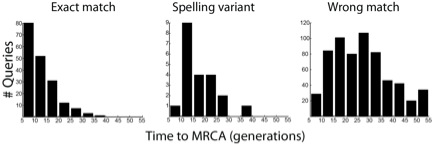
\includegraphics[width=0.65\textwidth]{Figures/App1/SuppFig1.jpg}
\end{figure}
\textbf{The TMRCA profiles of haplotype queries.} Records that matched exactly the input surname (left) showed a geometric-like distribution. For most records with a minute spelling variant from the original surname (center) the  MRCA was 10-15 generations ago. Wrong matches (right) mainly showed an ancient MRCA.

\pagebreak
\subsection{Supplemental Figure 2}
\begin{figure}[h!]
\centering
\label{fig:sursup2}
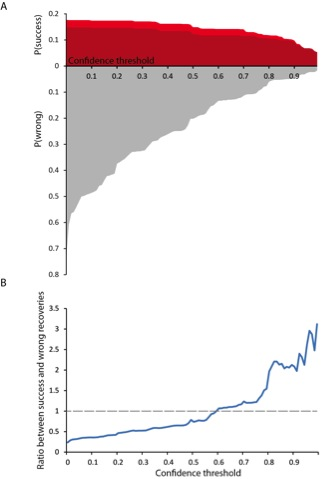
\includegraphics[width=0.4\textwidth]{Figures/App1/SuppFig2.jpg}
\end{figure}
\textbf{Performance of surname recovery at different confidence thresholds.} \textbf{(A)} The rate of successful recovery with exact matches (dark red) and spelling variants (light red) versus the wrong recovery rate (gray) as a function of confidence threshold level. \textbf{(B)} The ratio between successful recoveries to wrong recoveries.

\pagebreak
\subsection{Supplemental Figure 3}
\begin{figure}[h!]
\centering
\label{fig:sursup3}
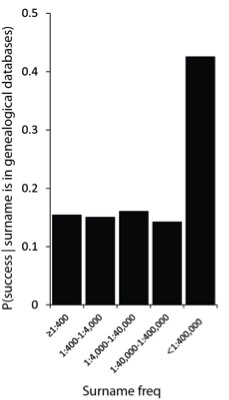
\includegraphics[width=0.4\textwidth]{Figures/App1/SuppFig3.jpg}
\end{figure}
\textbf{The probability of successful recovery given that the surname has at least one record in Ysearch or SMGF as a function of the surname frequency.}

\pagebreak
\subsection{Supplemental Figure 4}
\begin{figure}[h!]
\centering
\label{fig:sursup4}
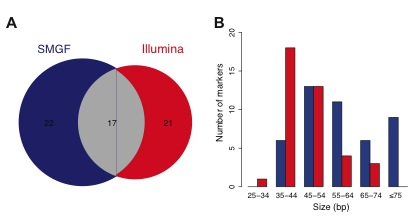
\includegraphics[width=0.65\textwidth]{Figures/App1/SuppFig4.jpg}
\end{figure}
\textbf{Comparison between Illumina Y-STR profiling and the Sorenson Genomics genetic genealogy service.} \textbf{(A)} Illumina profiling returned the results of 38 Y-STR markers. The genetic genealogy service uses a panel of 49 markers, 39 of which are included in lobSTR's Y-STR reference. The results of all 17 markers that were profiled by both strategies were identical. \textbf{(B)} The distribution of total STR region lengths is shown for the markers typed by Sorenson (blue) versus markers typed by lobSTR (red).

\pagebreak
\subsection{Supplemental Figure 5}
\begin{figure}[h!]
\centering
\label{fig:sursup5}
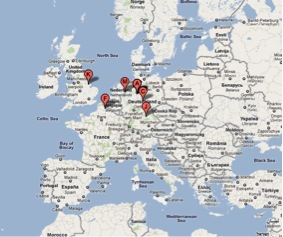
\includegraphics[width=0.65\textwidth]{Figures/App1/SuppFig5a.jpg}
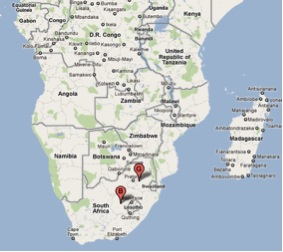
\includegraphics[width=0.65\textwidth]{Figures/App1/SuppFig5b.jpg}
\end{figure}
\textbf{Ancestral origins of Venter records in Ysearch}. The ancestral origin of the top match is labeled with an arrow.

\pagebreak
\subsection{Supplemental Figure 6}
\begin{figure}[h!]
\centering
\label{fig:sursup6}
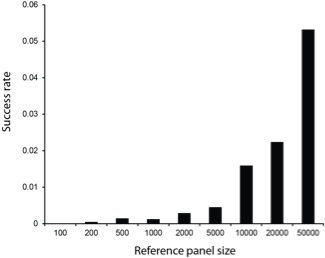
\includegraphics[width=0.65\textwidth]{Figures/App1/SuppFig6.jpg}
\end{figure}
\textbf{The estimated success rate for surname recovery after imputation as a function of the imputation panel size.}

\pagebreak
\section{Supplemental Tables}
\subsection{Supplemental Table 1}
\begin{figure}[h!]
\centering
\label{tab:sursuptab1} % even though we use a figure screenshot
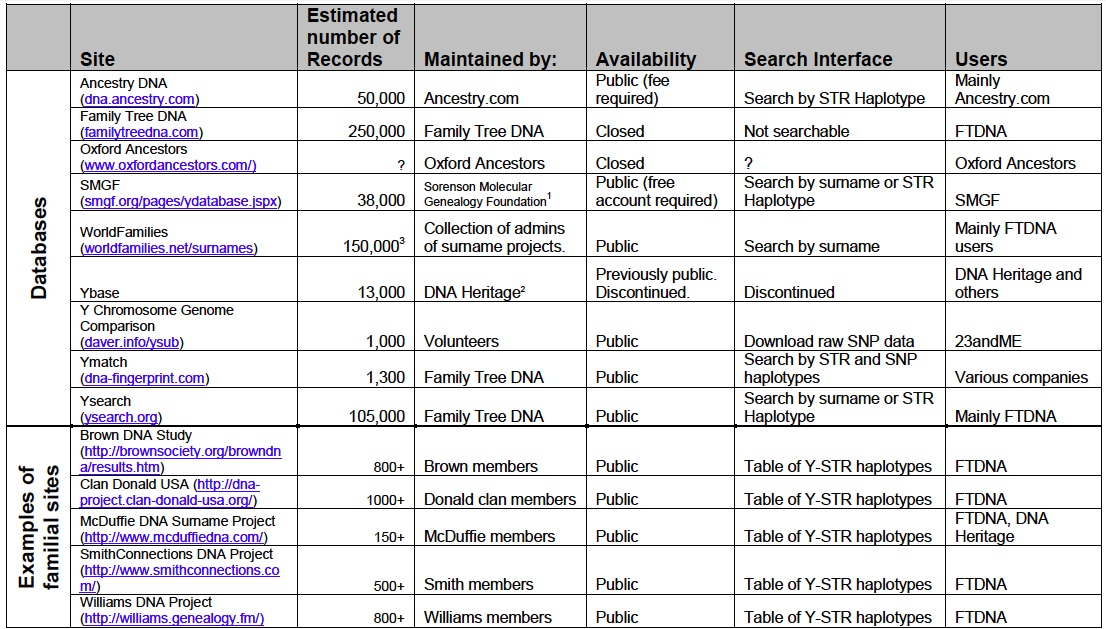
\includegraphics[width=0.95\textwidth]{Figures/App1/SuppTab1.jpg}
\end{figure}
List of major genetic genealogy sites that display Y chromosome and surname information. The top section lists genetic genealogy databases. The bottom section lists examples of privately maintained familial genetic genealogy sites.
$^1$ SMGF was recently acquired by Ancestry.com. $^2$ DNA Heritage was acquired by FamilyTreeDNA in 2011. $^3$ Includes only users whose surnames are present in the 2000 US Census.

\pagebreak
\subsection{Supplemental Table 2}
\begin{table}[h!]
\centering
\label{tab:sursuptab2}
\begin{adjustbox}{height=0.4\textheight}
\begin{tabular}{l l l l}
\hline
Marker & Expected mutation rate & Mean & $\sigma$ \\
\hline
DYS19     & 0.00437  & 14.34   & 0.8045 \\
DYS385a   & 0.00208  & 12.0869 & 1.6522 \\
DYS385b   & 0.00414  & 14.5464 & 1.449  \\
DYS388    & 0.000425 & 12.5142 & 1.0753 \\
DYS389a   & 0.00551  & 12.9668 & 0.6644 \\
DYS389b   & 0.00383  & 29.326  & 1.0418 \\
DYS390    & 0.00152  & 23.6032 & 1.0229 \\
DYS391    & 0.00323  & 10.4858 & 0.6104 \\
DYS392    & 0.00097  & 12.3413 & 1.1069 \\
DYS393    & 0.00211  & 13.0752 & 0.6025 \\
DYS426    & 0.000398 & 11.6459 & 0.5198 \\
DYS437    & 0.00153  & 14.9094 & 0.6931 \\
DYS438    & 0.000956 & 11.2206 & 1.0643 \\
DYS439    & 0.00384  & 11.66   & 0.8567 \\
DYS442    & 0.00978  & 17.2273 & 1.3301 \\
DYS444    & 0.00545  & 12.3666 & 0.892  \\
DYS445    & 0.00216  & 11.6015 & 0.9401 \\
DYS446    & 0.00267  & 13.1767 & 1.372  \\
DYS447    & 0.00212  & 24.6396 & 1.2057 \\
DYS448    & 0.000394 & 19.3437 & 0.8748 \\
DYS449    & 0.0122   & 29.5472 & 1.6474 \\
DYS452    & 0.00402  & 30.1854 & 1.1041 \\
DYS454    & 0.000475 & 11.0484 & 0.3744 \\
DYS455    & 0.000426 & 10.648  & 0.9704 \\
DYS456    & 0.00494  & 15.4571 & 1.1065 \\
DYS458    & 0.00836  & 16.6389 & 1.2634 \\
DYS459a   & 0.00013  & 8.753   & 0.5017 \\
DYS459b   & 0.00013  & 9.601   & 0.5422 \\
DYS460    & 0.00622  & 10.6976 & 0.639  \\
DYS461    & 0.000989 & 11.882  & 0.6914 \\
DYS462    & 0.00265  & 11.3571 & 0.6266 \\
DYS464a   & 0.00018  & 13.8555 & 1.4488 \\
DYS464b   & 0.00018  & 14.7374 & 1.0564 \\
DYS464c   & 0.00018  & 15.8236 & 1.124  \\
DYS464d   & 0.00018  & 16.5742 & 1.1157 \\
DYS635    & 0.00385  & 22.6604 & 1.1601 \\
GATA-A10  & 0.00332  & 15.5234 & 1.2242 \\
GATA-H4   & 0.00322  & 10.7333 & 0.7801 \\
GGAAT1B07 & 0.0024   & 10.2854 & 0.7397 \\
YCAIIa    & 0.002    & 19.0997 & 0.905  \\
YCAIIb    & 0.002    & 22.136  & 1.2624 \\
\hline
\end{tabular}
\end{adjustbox}
\caption{\textbf{List of markers used to challenge Ysearch and SMGF.} Mutation rates are based on Ballantyne et al. \cite{BallantyneGoedbloedFangEtAl2010}. YCAII was absent from this study and set to 0.002 according to Walsh \cite{Walsh2001}. Mean and standard deviations for marker values are calculated using Ysearch with NIST nomenclature.}
\end{table}

\pagebreak
\subsection{Supplemental Table 3}
\label{tab:sursuptab3}
\begin{tabularx}{\linewidth}{l l l l l l }
\hline
Marker & Start & End & Alt location & Ref allele & Motif structure \\
\hline
DYS394/19   & 9521989  & 9522052  &                        & 15 & {[}TAGA{]}3TAGG{[}TAGA{]}n                                                                                                           \\
DYS385a/b   & 20842518 & 20842573 & chrY:19260956-19261212 & 14 & {[}GAAA{]}n                                                                                                                          \\
DYS388      & 14747535 & 14747570 &                        & 12 & {[}ATT{]}n                                                                                                                           \\
DYS389I     & 14612191 & 14612238 &                        & 12 & {[}TCTG{]}m{[}TCTA{]}n                                                                                                               \\
DYS389B     & 14612338 & 14612405 &                        & 29 & {[}TCTG{]}m{[}TCTA{]}n                                                                                                               \\
DYS390      & 17274947 & 17275042 &                        & 24 & {[}TCTG{]}n{[}TCTA{]}m{[}TCTG{]}p{[}TCTA{]}q                                                                                         \\
DYS391      & 14102795 & 14102838 &                        & 11 & {[}TCTA{]}n                                                                                                                          \\
DYS392      & 22633873 & 22633911 &                        & 13 & {[}TAT{]}n                                                                                                                           \\
DYS393      & 3131152  & 3131199  &                        & 12 & {[}AGAT{]}n                                                                                                                          \\
DYS406S1    & 23843595 & 23843634 &                        & 10 & {[}TATC{]}n                                                                                                                          \\
DYS413a/b   & 16099088 & 16099133 & chrY:14676647-14676820 & 23 & {[}TG{]}n                                                                                                                            \\
DYS426      & 19134850 & 19134885 &                        & 12 & {[}GTT{]}n                                                                                                                           \\
DYS434      & 14466533 & 14466568 &                        & 9  & TAAT{[}CTAT{]}n                                                                                                                      \\
DYS435      & 14496298 & 14496333 &                        & 9  & {[}TGGA{]}n                                                                                                                          \\
DYS436      & 15203862 & 15203897 &                        & 12 & {[}GTT{]}n                                                                                                                           \\
DYS437      & 14466994 & 14467057 &                        & 16 & {[}TCTA{]}n{[}TCTG{]}2{[}TCTA{]}4                                                                                                    \\
DYS438      & 14937824 & 14937873 &                        & 10 & {[}TTTTC{]}n                                                                                                                         \\
DYS439      & 14515312 & 14515363 &                        & 13 & {[}GATA{]}n                                                                                                                          \\
DYS441      & 14981831 & 14981908 &                        & 16 & {[}TTCC{]}n                                                                                                                          \\
DYS442      & 14761103 & 14761168 &                        & 17 & {[}TATC{]}2{[}TGTC{]}3{[}TATC{]}n                                                                                                    \\
DYS444      & 19226192 & 19226247 &                        & 14 & {[}TAGA{]}n                                                                                                                          \\
DYS445      & 22092602 & 22092649 &                        & 12 & {[}TTTA{]}n                                                                                                                          \\
DYS446      & 3131458  & 3131527  &                        & 14 & {[}TCTCT{]}n                                                                                                                         \\
DYS447      & 15278740 & 15278854 &                        & 23 & {[}TAATA{]}n{[}TAAAA{]}1{[}TAATA{]}m{[}TAAAA{]}1{[}TAATA{]}p                                                                         \\
DYS448\_1   & 24365070 & 24365136 &                        & 11 & {[}AGAGAT{]}n                                                                                                                        \\
DYS448\_2   & 24365178 & 24365225 &                        & 8  & {[}AGAGAT{]}n                                                                                                                        \\
DYS449\_1   & 8218014  & 8218074  &                        & 13 & {[}TTTC{]}n                                                                                                                          \\
DYS449\_2   & 8218124  & 8218179  &                        & 14 & {[}TTTC{]}n                                                                                                                          \\
DYS450      & 8126300  & 8126344  &                        & 8  & {[}ATTTT{]}n                                                                                                                         \\
DYS452      & 21620478 & 21620632 &                        & 31 & {[}TATAC{]}m{[}TGTAC{]}n{[}TATAC{]}p{[}CATAC{]}{[}TATAC{]}{[}CATAC{]}{[}TATAC{]}q{[}CATAC{]}r{[}TATAC{]}s{[}CATAC{]}{[}TATAC{]}t     \\
DYS454      & 8224156  & 8224199  &                        & 11 & {[}AAAT{]}n                                                                                                                          \\
DYS455      & 6911569  & 6911612  &                        & 11 & {[}AAAT{]}n                                                                                                                          \\
DYS456      & 4270960  & 4271019  &                        & 15 & {[}AGAT{]}n                                                                                                                          \\
DYS458      & 7867880  & 7867943  &                        & 16 & {[}GAAA{]}n                                                                                                                          \\
DYS459a/b   & 26078851 & 26078890 & chrY:26292857-26293004 & 10 & {[}TAAA{]}n                                                                                                                          \\
DYS460      & 21050842 & 21050881 &                        & 10 & {[}ATAG{]}n                                                                                                                          \\
DYS461      & 21050690 & 21050737 &                        & 12 & {[}TAGA{]}n{[}CAGA{]}                                                                                                                \\
DYS462      & 21317047 & 21317090 &                        & 11 & {[}TATG{]}n                                                                                                                          \\
DYS463      & 7643509  & 7643628  &                        & 24 & {[}AAAGG{]}m {[}AAGGG{]}n {[}AAGGA{]}p                                                                                               \\
DYS472      & 16508484 & 16508507 &                        & 8  & {[}AAT{]}n                                                                                                                           \\
DYS481      & 8426378  & 8426443  &                        & 22 & {[}CTT{]}n                                                                                                                           \\
DYS485      & 22099634 & 22099681 &                        & 16 & {[}TTA{]}n                                                                                                                           \\
DYS487      & 8914174  & 8914212  &                        & 13 & {[}TTA{]}n                                                                                                                           \\
DYS490      & 3443765  & 3443800  &                        & 12 & {[}TTA{]}n                                                                                                                           \\
DYS492      & 17414337 & 17414369 &                        & 12 & {[}ATT{]}n                                                                                                                           \\
DYS494      & 21386168 & 21386197 &                        & 10 & {[}TTA{]}n                                                                                                                           \\
DYS495      & 15011300 & 15011346 &                        & 15 & {[}AAT{]}n                                                                                                                           \\
DYS505      & 3640831  & 3640878  &                        & 12 & {[}TCCT{]}n                                                                                                                          \\
DYS511      & 17304923 & 17304958 &                        & 10 & {[}GATA{]}n                                                                                                                          \\
DYS520      & 7730432  & 7730511  &                        & 20 & {[}ATAG{]}n{[}ATAC{]}n                                                                                                               \\
DYS522      & 7415625  & 7415664  &                        & 10 & {[}GATA{]}n                                                                                                                          \\
DYS531      & 8466195  & 8466238  &                        & 11 & {[}AAAT{]}n                                                                                                                          \\
DYS533      & 18393226 & 18393273 &                        & 12 & {[}ATCT{]}n                                                                                                                          \\
DYS634      & 18392976 & 18393035 &                        & 15 & {[}CTTT{]}n                                                                                                                          \\
DYS537      & 19358850 & 19358889 &                        & 10 & {[}TCTA{]}n                                                                                                                          \\
DYS549      & 21520224 & 21520275 &                        & 13 & {[}GATA{]}n                                                                                                                          \\
DYS556      & 22601453 & 22601496 &                        & 11 & {[}AATA{]}n                                                                                                                          \\
DYS557      & 23234712 & 23234775 &                        & 16 & {[}TTTC{]}n                                                                                                                          \\
DYS565      & 16526732 & 16526775 &                        & 12 & {[}ATAA{]}n                                                                                                                          \\
DYS568      & 8822555  & 8822594  &                        & 11 & {[}AAAT{]}n                                                                                                                          \\
DYS570      & 6861231  & 6861298  &                        & 17 & {[}TTTC{]}n                                                                                                                          \\
DYS572      & 3679660  & 3679699  &                        & 10 & {[}AAAT{]}n                                                                                                                          \\
DYS575      & 7436257  & 7436296  &                        & 10 & {[}AAAT{]}n                                                                                                                          \\
DYS576      & 7053359  & 7053426  &                        & 16 & {[}AAAG{]}n                                                                                                                          \\
DYS578      & 22562564 & 22562599 &                        & 9  & {[}AAAT{]}n                                                                                                                          \\
DYS589      & 24485693 & 24485757 &                        & 12 & {[}TTTTA{]}n                                                                                                                         \\
DYS590      & 8555980  & 8556019  &                        & 8  & {[}TTTTG{]}n                                                                                                                         \\
DYS594      & 21656837 & 21656886 &                        & 10 & {[}AAATA{]}n                                                                                                                         \\
DYS607      & 18414382 & 18414457 &                        & 19 & {[}GAAG{]}n{[}GAAA{]}{[}GAAG{]}{[}GAAA{]}{[}GAAG{]}                                                                                  \\
DYS617      & 19081518 & 19081553 &                        & 12 & {[}TTAn{]}                                                                                                                           \\
DYS635      & 14379564 & 14379655 &                        & 23 & {[}TCTA{]}4{[}TGTA{]}2{[}TCTA{]}2{[}TGTA{]}2{[}TCTA{]}2{[}TGTA{]}m{[}TCTA{]}n                                                        \\
DYS636      & 22634857 & 22634900 &                        & 12 & {[}ATTT{]}n                                                                                                                          \\
DYS638      & 17645491 & 17645534 &                        & 11 & {[}TTTA{]}n                                                                                                                          \\
DYS641      & 16134296 & 16134335 &                        & 10 & {[}TAAA{]}n                                                                                                                          \\
DYS643      & 17426012 & 17426066 &                        & 11 & {[}CTTTT{]}n                                                                                                                         \\
DYS714      & 22147731 & 22147865 &                        & 27 & {[}TTTCT{]}m{[}CTTCT{]}n{[}TTTCT{]}p{[}CTTCT{]}q{[}TTTCT{]}r                                                                         \\
DYS717      & 17313245 & 17313324 &                        & 16 & {[}GTACT{]}m {[}GTATT{]}n                                                                                                            \\
GATA-A10    & 18718879 & 18718938 &                        & 15 & {[}TCCA{]}2 {[}TATC{]}n                                                                                                              \\
GATA-H4     & 18743553 & 18743600 &                        & 12 & {[}TAGA{]}n                                                                                                                          \\
YCAIIa/b    & 19622111 & 19622156 & chrY:19016986-19017135 & 23 & {[}CA{]}n                                                                                                                            \\
DYS395S1a/b & 19739341 & 19739381 & chrY:18899736-18899977 & 15 & {[}AAC{]}n                                                                                                                           \\
DYS716      & 13140129 & 13140274 &                        & 28 & {[}ACTCGC{]}{[}ACTCC{]}m{[}ATTCC{]}n{[}TATTCTATTGA{]}{[}ACTCC{]}{[}ATTCC{]}{[}ACTCC{]}2{[}ATTCA{]}{[}ATTCC{]}2{[}ACTTC{]}{[}ATTCC{]} \\
\hline
\end{tabularx}
\textbf{Y-STR genomic locations and conventions.} All coordinates are given for human genome build hg19. Conventions follow NIST guidelines whenever available. $^*$ The values for DYS448 and DYS449 were determined by adding the alleles typed at DYS448\_1/DYS448\_2 and DYS449\_1/DYS449\_2. The complete repeat structures for DYS448 and DYS449 are  [AGAGAT]mN42[AGAGAT]n and [TTTC]m [N]50 [TTTC]n, respectively.

\pagebreak
\subsection{Supplemental Table 4}
\label{tab:sursuptab4}
\begin{tabularx}{\linewidth}{l l l l}
\hline
Marker & Craig Venter & Best Ysearch hit (VPBT4) \\
\hline
DYS388    & 12 & 12 \\
DYS391    & 10 & 10 \\
DYS392    & 13 & 13 \\
DYS395S1a & 15 & 15 \\
DYS395S1b & 16 & 16 \\
DYS413a   & 23 & 23 \\
DYS426    & 12 & 12 \\
DYS436    & 12 & 12 \\
DYS438    & 12 & 12 \\
DYS439    & 12 & 12 \\
DYS442    & 12 & 12 \\
DYS450    & 8  & 8  \\
DYS454    & 11 & 11 \\
DYS455    & 11 & 11 \\
DYS458    & 17 & 17 \\
DYS459a   & 9  & 9  \\
DYS461    & 12 &    \\
DYS462    & 11 &    \\
DYS472    & 8  & 8  \\
DYS481    & 22 & 22 \\
DYS485    & 16 &    \\
DYS492    & 13 & 13 \\
DYS494    & 9  &    \\
DYS531    & 12 & 12 \\
DYS534    & 16 & 16 \\
DYS537    & 10 & 10 \\
DYS549    & 12 &    \\
DYS556    & 11 &    \\
DYS557    & 16 & 16 \\
DYS565    & 12 & 12 \\
DYS568    & 11 & 11 \\
DYS570    & 17 & 17 \\
DYS578    & 9  & 9  \\
DYS590    & 9  & 9  \\
DYS594    & 10 & 10 \\
DYS617    & 12 & 12 \\
DYS636    & 12 &    \\
DYS638    & 11 &    \\
DYS641    & 10 & 10 \\
DYS714    & 25 & 25 \\
YCAIIa    & 19 & 19 \\
YCAIIb    & 23 & 23 \\
\hline
\end{tabularx}
\textbf{Craig Venter's haplotype from his personal genome versus the best Ysearch match.} Only Ysearch markers with corresponding sequencing results are shown. All alleles are reported using FamilyTreeDNA nomenclature to match the Ysearch convention. For Genebank read accessions, see Supplemental Material at \url{http://www.sciencemag.org/content/339/6117/321/suppl/DC1}.

\pagebreak
\subsection{Supplemental Table 5}
\begin{table}[h!]
\centering
\label{tab:sursuptab5}
\begin{adjustbox}{width=1\textwidth}
\begin{tabular}{l l l}
\hline
User surname & Ancestor surname & Origin \\
\hline
Venter & Von Dempter  & Hameln, Germany                                 \\
Venter & Venter       & Bloemfontein, South Africa                      \\
Venter & Venter       & Germany                                         \\
Venter & von Dempter  & Hamelin, Lower Saxony/Niedersachsen, Germany    \\
Venter & Von Dempter  & Hameln, Lower Saxony/Niedersachsen, Germany     \\
Venter & Venter       & Hamel, France                                   \\
Venter & Venter       & Witbank, South Africa                           \\
Venter & Von Dempter  & Hameln, Germany                                 \\
Venter & Venter       & Hamln, Germany                                  \\
Venter & Venter       & Roth near Meisenheim, Palatinate/Pfalz, Germany \\
Venter &              & Lincolnshire, England                           \\
Venter & Venter       & Hameln, Lower Saxony/Niedersachsen, Germany     \\
Venter & van Deventer & Oldenzee, Netherlands              \\
\hline
\end{tabular}
\end{adjustbox}
\caption{\textbf{Venter records in Ysearch and their ancestral origins.} In red - the top match to Craig Venter's Genome.}
\end{table}
